%%%%%%%%%%%%%%%%%%%%%%%%%%%%%%%%%%%%%%%%%
% Short Sectioned Assignment LaTeX Template Version 1.0 (5/5/12)
% This template has been downloaded from: http://www.LaTeXTemplates.com
% Original author:  Frits Wenneker (http://www.howtotex.com)
% License: CC BY-NC-SA 3.0 (http://creativecommons.org/licenses/by-nc-sa/3.0/)
%%%%%%%%%%%%%%%%%%%%%%%%%%%%%%%%%%%%%%%%%

% \documentclass[paper=a4, fontsize=11pt]{scrartcl} % A4 paper and 11pt font size
\documentclass[11pt, a4paper]{book}
\usepackage[T1]{fontenc} % Use 8-bit encoding that has 256 glyphs
\usepackage[utf8]{inputenc}
\usepackage{fourier} % Use the Adobe Utopia font for the document - comment this line to return to the LaTeX default
\usepackage{listings} % para insertar código con formato similar al editor
\usepackage[spanish, es-tabla]{babel} % Selecciona el español para palabras introducidas automáticamente, p.ej. "septiembre" en la fecha y especifica que se use la palabra Tabla en vez de Cuadro
\usepackage{url} % ,href} %para incluir URLs e hipervínculos dentro del texto (aunque hay que instalar href)
\usepackage{graphics,graphicx, float} %para incluir imágenes y colocarlas
\usepackage[gen]{eurosym} %para incluir el símbolo del euro
\usepackage{cite} %para incluir citas del archivo <nombre>.bib
\usepackage{enumerate}
\usepackage{hyperref}
\usepackage{graphicx}
\usepackage{tabularx}
\usepackage{booktabs}
\usepackage{pdflscape}

\usepackage[table,xcdraw]{xcolor}
\hypersetup{
	colorlinks=true,	% false: boxed links; true: colored links
	linkcolor=black,	% color of internal links
	urlcolor=cyan		% color of external links
}
\renewcommand{\familydefault}{\sfdefault}
\usepackage{fancyhdr} % Custom headers and footers
\pagestyle{fancyplain} % Makes all pages in the document conform to the custom headers and footers
\fancyhead[L]{} % Empty left header
\fancyhead[C]{} % Empty center header
\fancyhead[R]{José Pablo Márquez Megías} % My name
\fancyfoot[L]{} % Empty left footer
\fancyfoot[C]{} % Empty center footer
\fancyfoot[R]{\thepage} % Page numbering for right footer
%\renewcommand{\headrulewidth}{0pt} % Remove header underlines
\renewcommand{\footrulewidth}{0pt} % Remove footer underlines
\setlength{\headheight}{13.6pt} % Customize the height of the header

\usepackage{titlesec, blindtext, color}
\definecolor{gray75}{gray}{0.75}
\newcommand{\hsp}{\hspace{20pt}}
\titleformat{\chapter}[hang]{\Huge\bfseries}{\thechapter\hsp\textcolor{gray75}{|}\hsp}{0pt}{\Huge\bfseries}
\setcounter{secnumdepth}{4}
\usepackage[Lenny]{fncychap}


\begin{document}

	% Plantilla portada UGR
	\begin{titlepage}
\newlength{\centeroffset}
\setlength{\centeroffset}{-0.5\oddsidemargin}
\addtolength{\centeroffset}{0.5\evensidemargin}
\thispagestyle{empty}

\noindent\hspace*{\centeroffset}\begin{minipage}{\textwidth}

\centering
\includegraphics[width=0.9\textwidth]{logos/logo_ugr.jpg}\\[1.4cm]

\textsc{ \Large TRABAJO FIN DE GRADO\\[0.2cm]}
\textsc{ GRADO EN INGENIERIA INFORMATICA}\\[1cm]

{\huge\bfseries Plataforma para la gestión de calendarios académicos basada en servicios web \\}
\noindent\rule[-1ex]{\textwidth}{3pt}\\[3.5ex]
{\large\bfseries GAC: Gestor Académico de Calendarios}\\
\vspace{1cm}
\textbf{Autor}\\ {José Pablo Márquez Megías}\\[2.5ex]
\textbf{Directores}\\ {Ángel Ruiz Zafra\\Kawtar Benghazi Akhlaki Sekkate}\\[2cm]
\includegraphics[width=0.3\textwidth]{logos/etsiit_logo.png}\\[0.1cm]
\textsc{Escuela Técnica Superior de Ingenierías Informática y de Telecomunicación}\\
\textsc{---}\\
Granada, septiembre de 2024
\end{minipage}
\end{titlepage}



	% Plantilla prefacio UGR
	\thispagestyle{empty}

\begin{center}
	\newpage
{\large\bfseries Plataforma para la gestión de calendarios académicos basada en servicios web}\\
\end{center}
\begin{center}
José Pablo Márquez Megías\\
\end{center}

%\vspace{0.7cm}

\vspace{0.5cm}
\noindent\textbf{Palabras clave}: \textit{software libre}, \textit{timetabling}, \textit{application programming interfaces}, \textit{web scraping}, \textit{servicios web}, \textit{arquitectura orientada a servicios}
\vspace{0.7cm}

\noindent\textbf{Resumen}\\

Cada año los estudiantes deben matricularse en una serie de asignaturas, organizadas en teoría y prácticas con horarios distribuidos a lo largo de la semana. Este proceso de matrícula, aunque fundamental, puede ser tedioso y propenso a errores, especialmente para aquellos con asignaturas pendientes de otros cursos o provenientes de ciclos formativos que deben combinar asignaturas de distintos cursos y grupos en un mismo cuatrimestre.\newline

El presente proyecto describe el desarrollo de una plataforma para la gestión de calendarios académicos, que permite a los estudiantes de la Universidad de Granada generar de forma automática un calendario semanal a partir de las asignaturas y grupos en los que deseen matricularse. La plataforma, denominada \textbf{GAC} (Gestor Académico de Calendarios), centraliza y mantiene actualizada toda la información relevante sobre la planificación docente, además de aportar una serie de herramientas que permiten a los alumnos la planificación automática de su selección de matrícula reduciendo significativamente el tiempo que les tomaría hacerlo de forma manual y sin errores.\newline

\cleardoublepage

\begin{center}
	{\large\bfseries Platform for the management of academic calendars based on web services}\\
\end{center}
\begin{center}
	José Pablo Márquez Megías\\
\end{center}
\vspace{0.5cm}
\noindent\textbf{Keywords}: \textit{open source}, \textit{timetabling}, \textit{web services}, \textit{application programming interfaces}, \textit{web scraping}, \textit{service-oriented architecture}
\vspace{0.7cm}

\noindent\textbf{Abstract}\\

Each year students must enroll in a series of subjects, organized in theory and practice with schedules distributed throughout the week. This enrollment process, although fundamental, can be tedious and error-prone, especially for those students with pending subjects from other courses or those coming from training cycles who must combine subjects from different courses and groups in the same term.\newline

This project describes the development of a platform for the management of academic calendars, which allows students at the University of Granada to automatically generate a weekly calendar based on the subjects and groups in which they wish to enroll. The platform, called GAC (Gestor Académico de Calendarios), centralizes and keeps updated all the relevant information about teaching planning, as well as providing a series of tools that allow students to automatically plan their enrollment selection, significantly reducing the time it would take them to do it manually and without errors.

\cleardoublepage

\thispagestyle{empty}

\noindent\rule[-1ex]{\textwidth}{2pt}\\[4.5ex]

D. \textbf{Ángel Ruíz Zafra} y Dª. \textbf{Kawtar Benghazi Akhlaki Sekkate}, Profesores del departamento de Lenguajes y Sistemas Informáticos.
\vspace{0.5cm}

\textbf{Informamos:}

\vspace{0.5cm}

Que el presente trabajo, titulado \textit{\textbf{Servicio web para la gestión de calendarios académicos}},
ha sido realizado bajo nuestra supervisión por \textbf{José Pablo Márquez Megías}, y autorizamos la defensa de dicho trabajo ante el tribunal
que corresponda.

\vspace{0.5cm}

Y para que conste, expiden y firman el presente informe en Granada a septiembre de 2024.

\vspace{1cm}

\textbf{El/la director(a)/es: }

\vspace{5cm}

\noindent \textbf{Ángel Ruíz Zafra} y \textbf{Kawtar Benghazi Akhlaki Sekkate}

\chapter*{Agradecimientos}

A mi familia, porque sin ellos no habría llegado hasta aquí. A mis amigos, por su apoyo incondicional. A mis tutores, por su paciencia y dedicación.


	% Índice de contenidos
	\newpage
	\tableofcontents

	% Índice de imágenes y tablas
	\newpage
	\listoffigures

	% Si hay suficientes se incluirá dicho índice
	\listoftables 
	\newpage

	% Introducción 
	\chapter{Introducción}
Entre las 27 facultades y escuelas \footnote[1]{\url{https://www.ugr.es/universidad/organizacion/facultades-escuelas}} que componen la universidad de Granada hay una oferta académica de 62 títulos de grado \footnote[2]{\url{https://www.ugr.es/destacado/oferta-academica-grados-masteres-y-doctorados}}. Los créditos totales que deben cursarse en la titulación serán de 240 ECTS \footnote[3]{\url{https://grados.ugr.es/documentacion/pages/infoacademica/estudios}}, distribuidos en 4 años. Los 60 pertenecientes a la formación básica se reparten entre 21 materias obligatorias (además del Trabajo Fin de Grado y las Prácticas Externas) y 13 optativas.\newline

Dichas asignaturas se imparten en grupos de teoría y sus correspondientes subgrupos de prácticas que se distribuyen en diferentes horarios a lo largo de la semana. Debido al modelo educativo vigente, el estudiante puede matricularse en varias asignaturas de distintos cursos simultáneamente. 

\section{Contexto y Motivación}
El uso de las TICS (Tecnologías de la Información y la Comunicación) se encuentra patente en entornos académicos y escolares. Estas tecnologías, a través de numerosas herramientas, mejoran significativamente los procesos de aprendizaje, la interacción entre profesor y estudiantado y, en definitiva, hacen mejor la experiencia educativa \cite{Flores-Alarcia2012} \cite{Paladines} \cite{TICenLaEducacion}.\newline

Dentro de estas herramientas, algunas se emplean para gestionar de forma eficiente, y en algunos casos de manera automática, tareas propias de personal administrativo, como el alta de nuevos estudiantes, registro de asignaturas, publicación de notas, etc. No obstante, a pesar el avance tecnológico, algunas tareas siguen realizándose manualmente, por la complicación que supone su automatización o bien por la falta de herramientas. Una tarea que aún se sigue realizando mayormente de manera manual es la generación de calendarios académicos personalizados.\newline

Todos los años el estudiante debe encargarse de consultar la información de las asignaturas en las que desea matricularse, así como los horarios de las clases y grupos de prácticas. A partir de esta información, el estudiante debe generar un calendario semanal que le permita visualizar de forma clara y concisa la distribución de las asignaturas. Esta tarea, aunque sencilla, puede resultar tediosa y propensa a errores, ya que el estudiante debe tener en cuenta la disponibilidad, los solapamientos de horarios, etc.\newline

Una vez pasado el proceso de matriculación, secretaría se encarga de hacer una distribución equilibrada de los estudiantes en los grupos de teoría y prácticas que les han sido asignados. Dicha asignación depende de varios factores tales como la demanda de plazas, la nota media del expediente académico, etc. Por otro lado, se priorizan las solicitudes de los estudiantes que seleccionan grupos completos para sus asignaturas sobre los que eligen grupos sueltos. Dicho proceso responde, principalmente, a la necesidad de evitar solapamientos, pero no se ajusta en todos los casos a las preferencias del estudiante.\newline

En el caso de alumnos con materias pendientes o estudiantes provenientes de ciclos formativos, el proceso no es tan sencillo como matricularse en todas las asignaturas del año que estén cursando.
Si un estudiante de ciclo formativo tiene convalidadas gran parte de las asignaturas de un año, o tiene pendientes asignaturas de cursos anteriores, es presumible que querrá matricularse en asignaturas de cursos superiores o inferiores, a fin de no perder tiempo y ni dinero (por motivo de becas, por ejemplo). En este contexto, la tarea de organizar un calendario ya no es tan sencilla, más aún si se tiene que elegir un grupo concreto para convalidar unas prácticas aprobadas de años anteriores por ejemplo.\newline

La motivación de este proyecto surge de la necesidad de facilitar a los estudiantes de la Universidad de Granada la generación de un calendario académico semanal a partir de las asignaturas y grupos en los que deseen matricularse. Reduciendo así la carga de trabajo y el tiempo invertido en dicha tarea.


\section{Objetivos}
Dado el enfoque de este proyecto, se han establecido una serie de objetivos para la \textit{creación de una aplicación web que permita a los estudiantes de la Universidad de Granada, generar un calendario académico semanal a partir de las asignaturas y grupos de prácticas en los que deseen matricularse.}\newline

Para la consecución de este objetivo principal, se han establecido los siguientes objetivos específicos:
\begin{enumerate}
    \item Revisión de soluciones existentes para la generación automática de calendarios académicos. Tanto comerciales como proyectos de investigación.
    \item Estudio de técnicas de timetabling.
    \item Estudio del uso de IA generativa para la solución del problema de timetabling.
    \item Estudio de nuevas tecnologías y paradigmas de computación, tales como tecnologías web, arquitecturas orientadas a servicios, etc.
\end{enumerate}

	% Estado del arte
	% 	1. Crítica al estado del arte
	% 	2. Propuesta
	\chapter{Estado de la cuestión}

Esta sección tiene como objetivo discutir la efectividad de la IA generativa como motor de calendarios para \textbf{GAC} y analizar los algoritmos de timetabling existentes y sus aplicaciones en el ámbito universitario. Se discutirán las ventajas y limitaciones de las soluciones actuales y otros trabajos relacionados.

\section{IA generativa}

La \textit{IA generativa}\footnote{\url{https://cloud.google.com/use-cases/generative-ai?hl=es}} hace referencia al uso de modelos de inteligencia artificial para la creación de contenido, como texto, imágenes, audio, etc. Se basan en \textit{modelos fundacionales} \footnote{\url{https://aws.amazon.com/es/what-is/foundation-models/}} que son redes neuronales de aprendizaje profundo y que sirven como punto de partida para el desarrollo de modelos de \textit{machine learning}. La IA generativa usa un modelo de aprendizaje automático para aprender patrones y relaciones dentro de un conjunto de datos creados por humanos. A partir de dichos patrones aprendidos, genera contenido. Los modelos de IA generativa se utilizan en una amplia variedad de aplicaciones, como la creación de arte, la generación de texto, la creación de música y la producción de contenido multimedia. Estos modelos son capaces de generar contenido de alta calidad y realista, lo que los hace útiles en una amplia gama de aplicaciones. Como puede verse en la Figura \ref{fig:llm_vs_generative}, aunque los LLM (Modelos de Lenguaje a Gran Escala) son un tipo específico de IA generativa enfocado exclusivamente en la generación y comprensión de texto, los modelos generativos no se limitan a esta capacidad. Estos modelos tienen la versatilidad de generar contenido en una amplia gama de formatos, incluyendo imágenes, audio, video, y otros tipos de datos.

\begin{figure}[H]
    \centering
    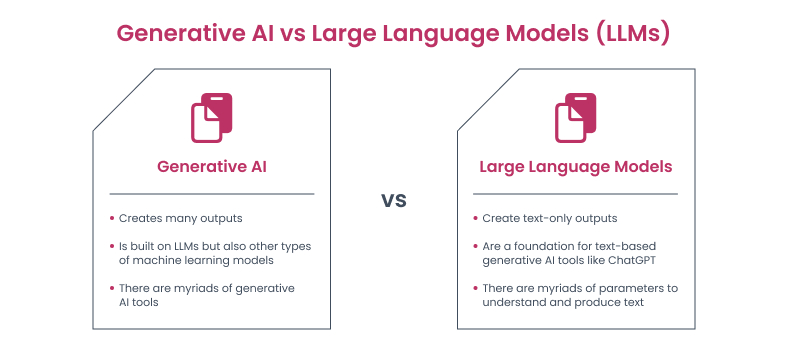
\includegraphics[width=1\textwidth]{./imagenes/large-language-models-vs-generative-ai-1.jpg}
    \caption{Diferencia entre LLM e IA Generativa \cite{chisw}.}
    \label{fig:llm_vs_generative}
\end{figure}


En un primer momento, era la opción escogida para llevar a cabo el backend de la plataforma \textbf{GAC}. Sin embargo, tras varias pruebas con diversos modelos como \emph{ChatGPT y Gemini}, se acabó descartando la idea dada la inconsistencia de los asistentes para organizar las clases de forma que no se solaparan y sin alterar los datos de los horarios proporcionados.

\subsection{Modelos utilizados}

A continuación se presentan los modelos de IA generativa utilizados en las pruebas realizadas para la generación de horarios:

\newcommand{\icon}[1]{\includegraphics[height=18pt]{#1}}
\subsubsection*{ChatGPT \protect\icon{./imagenes/ChatGPT_logo.png}}

Es un modelo de lenguaje de inteligencia artificial desarrollado por OpenAI\footnote{\url{https://chatgpt.com/}}. Es capaz de mantener conversaciones con los usuarios y responder preguntas en lenguaje natural. ChatGPT se basa en la arquitectura de transformadores y emplea el aprendizaje profundo para generar respuestas coherentes y relevantes. ChatGPT se puede utilizar en una variedad de aplicaciones, como asistentes virtuales, chatbots y sistemas de diálogo. ChatGPT es capaz de responder preguntas sobre una amplia gama de temas y proporcionar información útil a los usuarios. ChatGPT es una herramienta poderosa para la generación de lenguaje natural y la interacción con los usuarios en línea.

\renewcommand{\icon}[1]{\includegraphics[height=18pt]{#1}}
\subsubsection*{Gemini \protect\icon{./imagenes/gemini-icon.png}}

Es una familia de modelos de inteligencia artificial desarrollada por Google DeepMind\footnote{\url{https://gemini.google.com/app}}. Es la evolución de la tecnología detrás de \textbf{Bard}, integrando capacidades avanzadas de procesamiento de lenguaje natural con otros aspectos de la inteligencia artificial, como el razonamiento y la memoria. Gemini está diseñado para realizar tareas complejas que van más allá de la generación de texto, buscando mejorar la comprensión contextual, la generación de respuestas más precisas y la interacción más fluida con los usuarios. Es parte del esfuerzo de Google por mantenerse a la vanguardia en el desarrollo de IA generativa y cognitiva.

\subsection{Prompt Engineering}

Se refiere al diseño sistemático y la optimización de las instrucciones de entrada para guiar las respuestas de los LLM, garantizando la precisión, relevancia y coherencia de los resultados generados. Este proceso es crucial para aprovechar todo el potencial de estos modelos, haciéndolos más accesibles y aplicables en diversos ámbitos \cite{chen2023unleashing}.\newline

Como puede verse la Figura \ref{fig:role_prompt}, se empleó el método del \textbf{Role-prompting} con los modelos. Dicha técnica consiste en proporcionar al modelo un rol específico. Este método es efectivo para guiar las respuestas del modelo hacia un objetivo concreto \cite{Zhang_2023}.\newline

\begin{figure}[H]
    \centering
    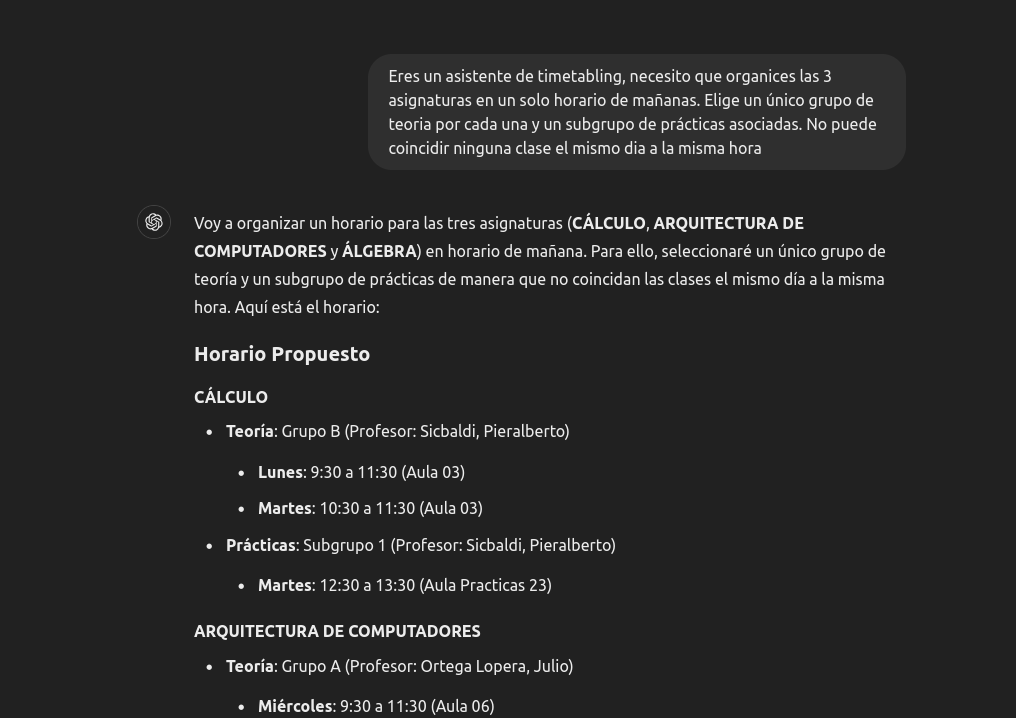
\includegraphics[width=1\textwidth]{./imagenes/Role_prompt.png}
    \caption{Ejemplo de Role-prompting con ChatGPT.}
    \label{fig:role_prompt}
\end{figure}

Además del método anterior, se siguieron los siguientes básicos del prompt Engineering \cite{Zhang_2023} para mejorar la calidad de las respuestas generadas por los modelos:

\subsubsection*{Dar instrucciones}
Se ha observado que las respuestas generadas por los modelos tienden a ser excesivamente generales cuando se le proporcionan instrucciones desprovistas de cualquier descripción suplementaria. Es imprescindible una descripción exhaustiva, como la de la Figura \ref{fig:contexto} para resultados más precisos.

\begin{figure}[H]
    \centering
    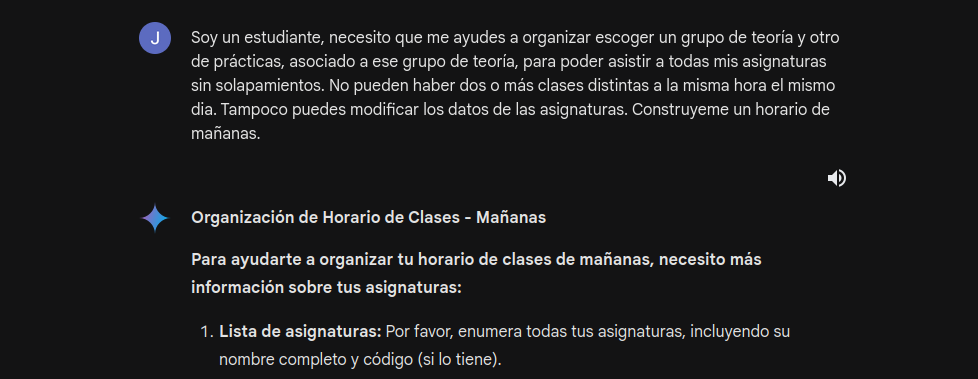
\includegraphics[width=1\textwidth]{./imagenes/Gemini_contexto.png}
    \caption{Ejemplo de instrucciónes descriptivas con Gemini.}
    \label{fig:contexto}
\end{figure}


\subsubsection*{Ser claro y preciso}
Los prompts deben estar exentos de ambigüedades y ser lo más específicos posible. Esto ayuda a los modelos a entender mejor el contexto y a generar respuestas más relevantes.

\subsubsection*{Intentarlo varias veces}
Debido a la naturaleza no determinista de los modelos basados en LLM, resulta beneficioso probar varias veces a la hora de generar respuestas. Esta técnica, denominada como ``remuestreo'' consiste en ejecutar varias veces el modelo con el mismo prompt y seleccionar la respuesta más adecuada.

\subsection{Resultados obtenidos}

A pesar de seguir las técnicas citadas anteriormente, los modelos de IA generativa no fueron capaces de generar horarios sin solapamientos ni omisiones. Aunque los datos proporcionados en forma de lenguaje natural y en formato JSON, fueron leeidos correctamente la mayoría de las veces, los modelos no pudieron organizar las clases de forma que se ajustaran a las restricciones del problema.\newline

A continuación se muestran en las Figuras \ref{fig:chatgpt} y \ref{fig:gemini} ejemplos de los resultados obtenidos con los modelos de IA generativa:

\begin{figure}[H]
    \centering
    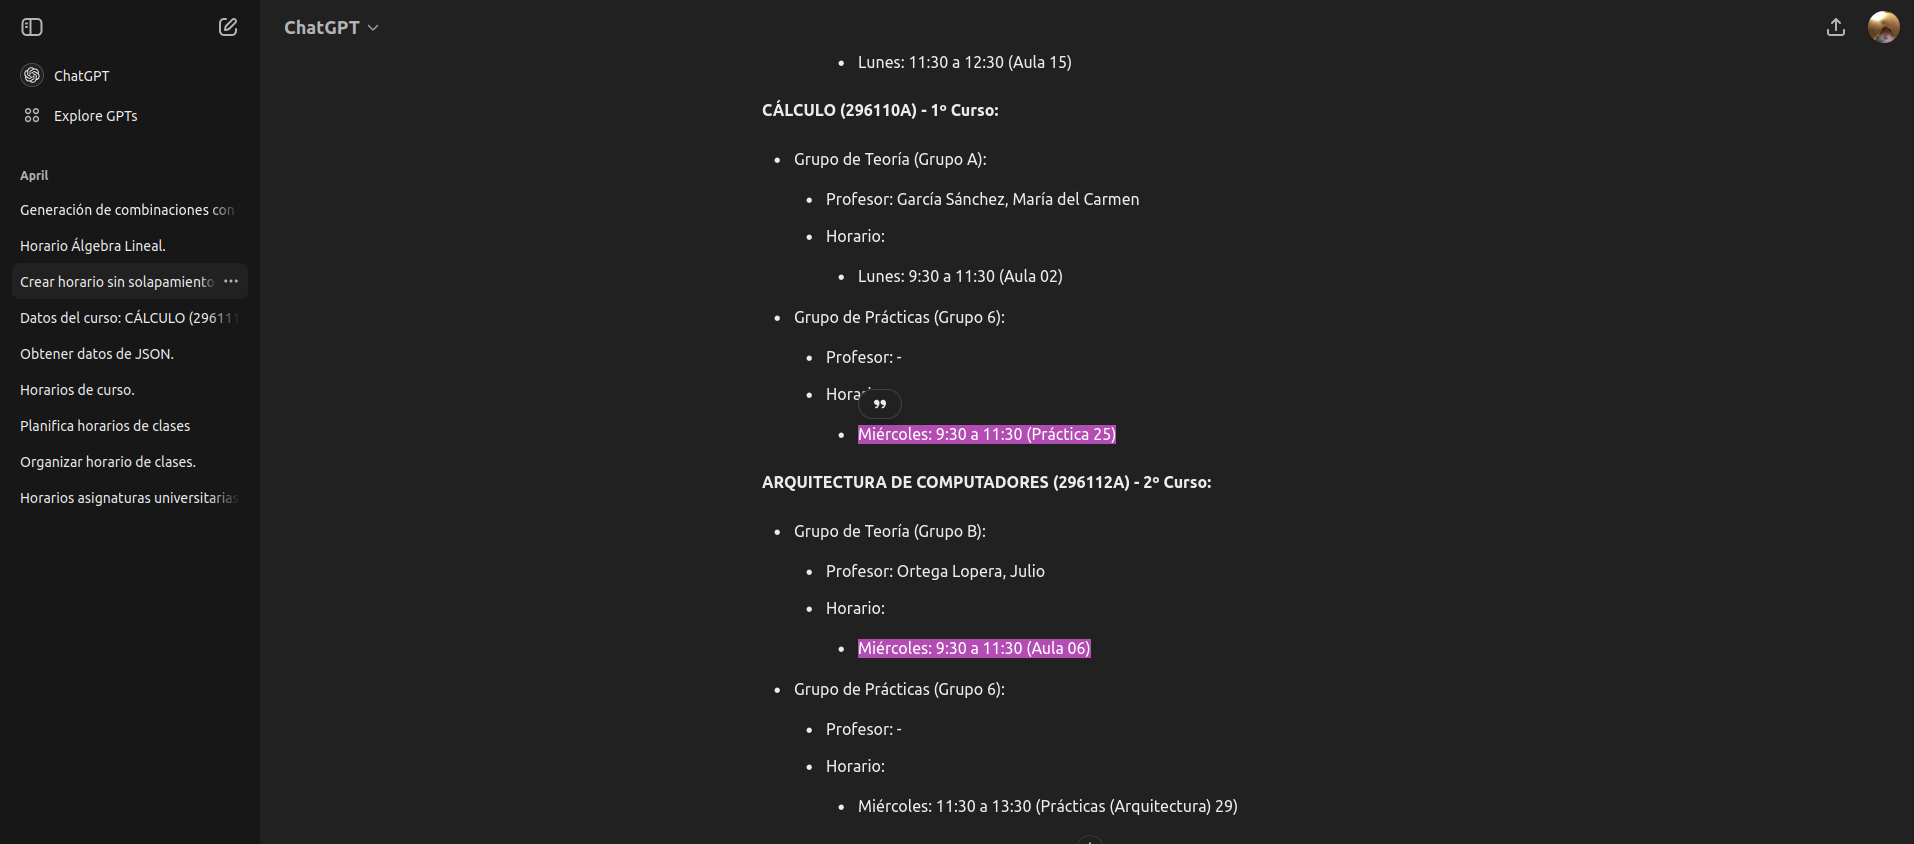
\includegraphics[width=1\textwidth]{./imagenes/ChatGPT.png}
    \caption{Ejemplo con ChatGPT 3.5: solapa las clases.}
    \label{fig:chatgpt}
\end{figure}

\begin{figure}[H]
    \centering
    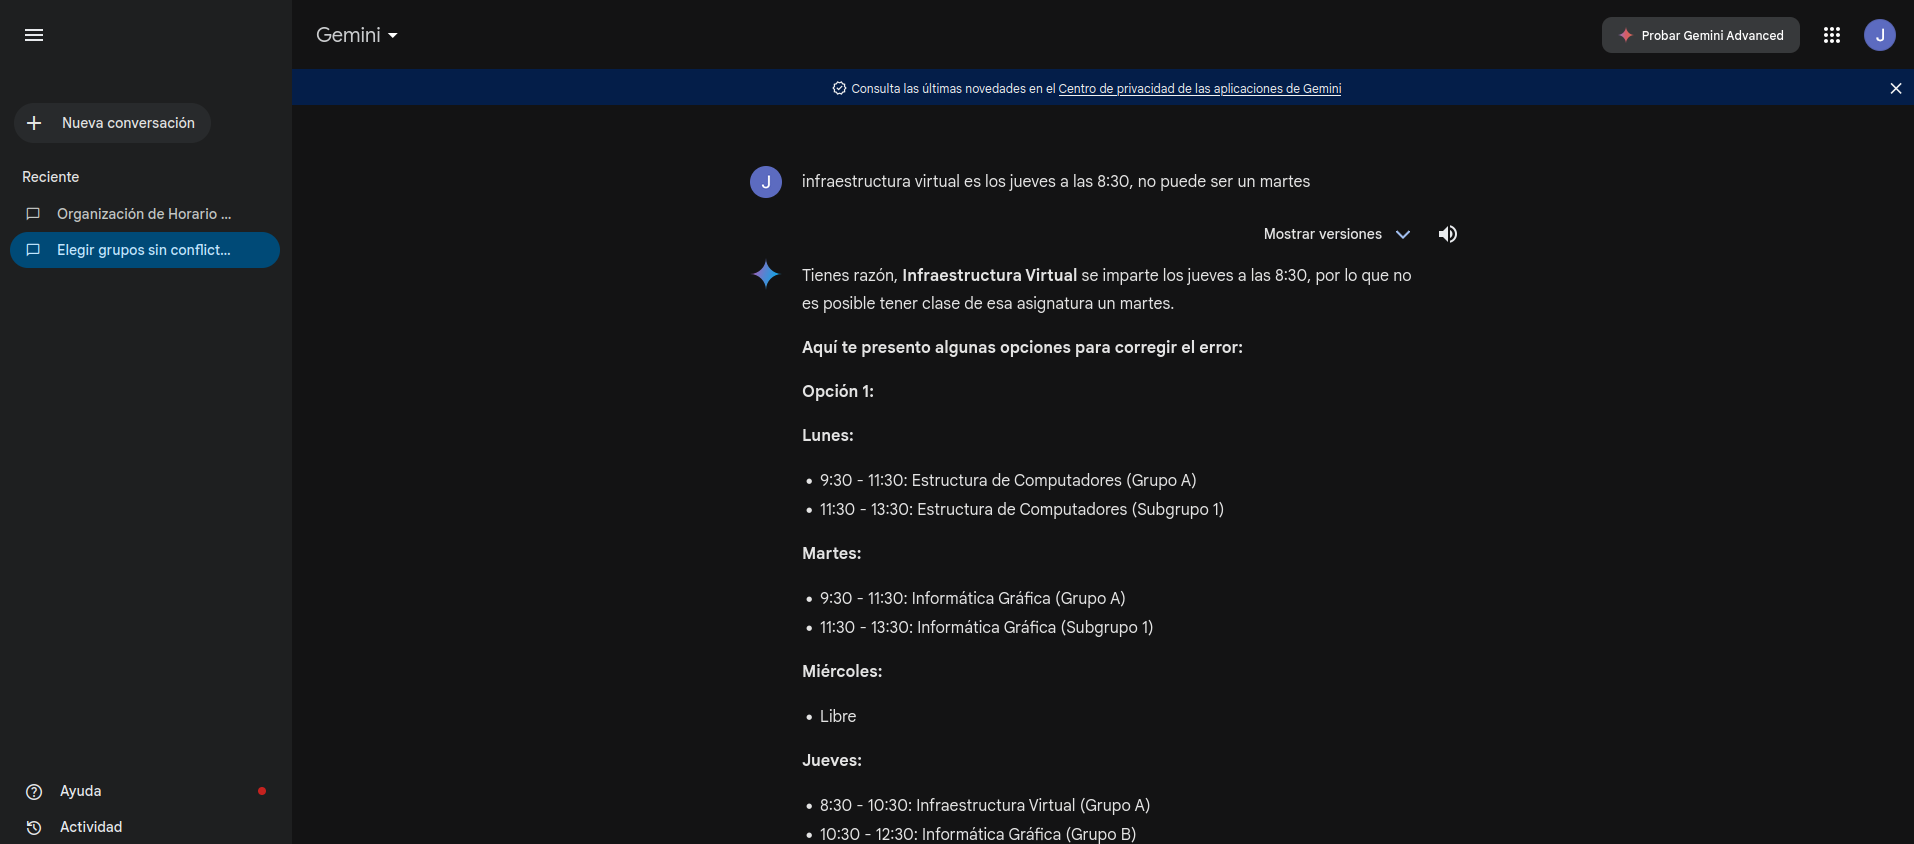
\includegraphics[width=1\textwidth]{./imagenes/Gemini.png}
    \caption{Ejemplo con Gemini (Bard): omite asignaturas.}
    \label{fig:gemini}
\end{figure}

\section{Algoritmos de timetabling}

El \textbf{timetabling} puede definirse generalmente como la actividad de asignar, con sujeción a restricciones, una serie de eventos a un número limitado de periodos de tiempo y lugares, de forma que se satisfagan los objetivos deseables en la medida de lo posible. Los casos prácticos en los que se plantea esta actividad son muy variados. En el ámbito educacional, empresarial, deportivo, de comunicación y transporte, entre otros \cite{hybrid-timetabling}.\newpage

Generalmente, en las instituciones de enseñanza son dos los problemas de timetabling que surgen: uno para \textbf{exámenes} (Examination Timetabling Problem) y el otro para la \textbf{programación de cursos} (Course Timetabling Problem y Class/Teacher Timetabling Problem o CTTP) \cite{carter}.\newline

\subsection{Examination Timetabling Problem}
El ETP básicamente involucra la asignación de una serie de exámenes a un período de examinación dado. Algunas versiones de este problema requieren que el calendario de la solución use el mínimo número de períodos de tiempo. Cada ETP tiene su propio conjunto de restricciones duras y restricciones blandas \cite{AutomatedTimetabling,NAJIAZIMI2005705}.\newline

Las restricciones duras deben ser satisfechas por el calendario. Por ejemplo, un estudiante no puede tener dos exámenes al mismo tiempo. Los calendarios que cumplen las restricciones duras se conocen como ``calendarios factibles''.\newline

Los requisitos blandos, por otra parte, son una lista de deseos con propiedades que se querría que los calendarios posean. Por ejemplo, no se acumularán en un mismo día varios exámenes de elevada dificultad y duración.\newline

El enfoque adoptado por los primeros intentos de resolver el ETP generalmente consistía en clasificar los exámenes según la dificultad asociada a la programación de los mismos y ordenando a estos como los primeros para evitar que se produjesen solapamientos. Desde entonces, múltiples avances se han producido en la resolución de este problema, incluyendo la aplicación de heurísticas y metaheurísticas, técnicas de construcción secuencial, algoritmos genéticos, etc.

A continuación se muestra en la Figura \ref{fig:IGA_ETP} un ejemplo de un algoritmo genético\footnote{Algoritmo Genético Interactivo (por sus siglas en inglés, Interactive Genetic Algorithm). Los IGAs son una variación de los algoritmos genéticos tradicionales que involucran la interacción humana en el proceso de optimización.} para resolver el ETP \cite{PILLAY2010457}:

\begin{figure}[H]
    \centering
    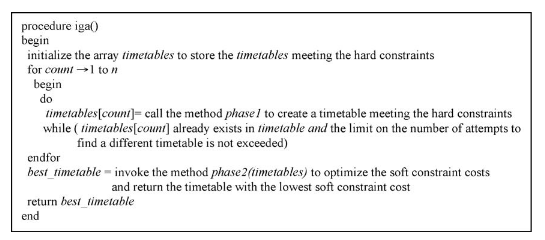
\includegraphics[width=1\textwidth]{./imagenes/IGA_ETP.png}
    \caption{Ejemplo de IGA para evolucionar calendarios ``factibles'' \cite{PILLAY2010457}.}
    \label{fig:IGA_ETP}
\end{figure}

% \newpage

% \begin{figure}
%     \begin{figure}[H]
%         \centering
%         \rotatebox{90}{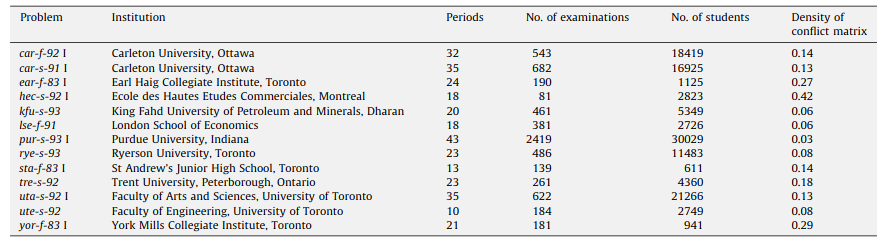
\includegraphics[width=1.5\textwidth]{./imagenes/IGA_Carter_Benchmarks.png}}
%         \caption{Benchmarks en los que fue probado el algoritmo de la figura anterior\cite{PILLAY2010457}.}
%     \end{figure}
% \end{figure}

\subsection{University Course TimeTabling Problem}

El UCTTP, es un problema de optimización\footnote{Es un problema que trata de calcular el valor máximo o mínimo de una función, en nuestro caso, de una variable. Por ejemplo: minimizar el error en una medición, minimizar la cantidad de material para construir un contenedor, maximizar el volumen de un contenedor, minimizar el tiempo de espera o de recorrido, etc.} híbrido que se presenta al comienzo de cada semestre de las universidades e incluye la asignación de eventos(\textbf{cursos}, profesores y estudiantes) a una serie de \textbf{franjas horarias} y salas fijas. Este problema debe satisfacer tanto las restricciones duras como las blandas durante la asignación de eventos a los recursos\footnote{Son usados por los eventos, tales como: salas, franjas de tiempo, etc.}, de modo que los posibles horarios se obtienen después de la plena satisfacción de todas las restricciones duras y también de las restricciones blandas para aumentar y promover la calidad de los posibles horarios generados según sea necesario \cite{UCTTP_ThreePhaseApproach}.\newline

El número de restricciones (duras y blandas) en este problema difiere de una institución a otra. Por lo tanto, el objetivo principal de todos los algoritmos mencionados es maximizar el número de restricciones blandas satisfechas en los horarios finales \cite{article_1445178}.\newline

Las restricciones del problema se clasifican en dos clases: duras y blandas. Las duras deben satisfacerse por completo en el problema para que la solución generada sea posible y sin conflictos; no se permite ninguna violación de estas restricciones. Las restricciones blandas están relacionadas con la función objetivo, la cual consiste en maximizar el número de restricciones blandas satisfechas. A diferencia de las restricciones duras, las blandas no tienen que satisfacerse necesariamente; pero a medida que aumenta el número de estas restricciones satisfechas, aumenta la calidad de las soluciones de dicha función. A continuación se presenta una lista de ejemplos de restricciones duras y blandas \cite{BABAEI201543}:

\begin{itemize}
    \item Un profesor no puede estar en dos lugares al mismo tiempo.
    \item Una clase no puede impartirse en dos salas al mismo tiempo.
    \item Un profesor imparte solo una clase a la vez.
    \item Un profesor puede solicitar un aula específica para una clase.
    \item El número máximo de horas que un profesor puede impartir en una clase son 4 horas.
    \item El máximo de horas que un alumno puede tener en un día son 4 horas.
    \item La hora de inicio de las clases puede ser las 8:00 a.m y la de finalización las 20:30 p.m. generalmente.
\end{itemize}
A continuación se muestra en la Figura \ref{fig:UCTTP} un ejemplo de un algoritmo para resolver el UCTTP mediante búsqueda iterativa en profundidad:

\begin{figure}[H]
    \centering
    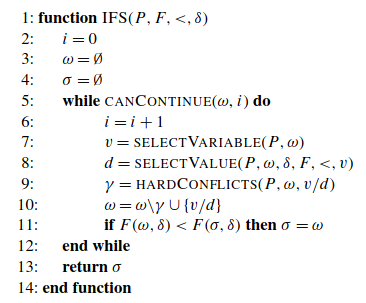
\includegraphics[width=0.7\textwidth]{./imagenes/UCTTP_Algoritmo.png}
    \caption{Pseudocódigo para algoritmo de UCTTP \cite{Rudova2011}.}
    \label{fig:UCTTP}
\end{figure}


\subsection{Class/Teacher Timetabling Problem}

El CTTP, suele encontrarse en escuelas con planes de estudios menos modulares. Tal es el caso de la mayoría de los institutos y algunas universidades, donde la mayoría de las lecciones predefinidas adscritas a cada curso son obligatorias para las respectivas clases. A diferencia del problema de programación de cursos, en el caso del CTTP \textbf{no se permite el solapamiento de lecciones}. En este caso, el objetivo consiste en programar el conjunto de lecciones satisfaciendo una serie de restricciones específicas de la institución \cite{doi:10.1504/IJOR.2024.139234}.\newline

Se han aplicado varias técnicas de resolución, desde
algoritmos basados en la teoría de grafos (de Werra 1996), a la programación binaria (Tri-pathy 1984; Birbas et al. 1997) y enfoques basados en restricciones (Yoshikawa et al. 1994). Además, las metaheurísticas basadas en el recocido simulado (Abramson 1982), las redes neuronales (Gislen et al. 1992), los algoritmos genéticos (Colorni et al. 1991) y la búsqueda tabú (Costa 1994) se han aplicado con éxito a casos concretos, objeto de estudio de los respectivos autores.\newline

En términos generales, el CTTP puede definirse como el problema de programar un conjunto de lecciones (una lección es una asignación previa de una o más clases rígidas de alumnos a un profesor y una asignatura) en un conjunto de periodos de tiempo y aulas adecuadas, satisfaciendo al mismo tiempo una amplia gama de restricciones. Estas pueden dividirse en dos niveles de importancia, como en los problemas de timetabling anteriores: restricciones duras y blandas \cite{carter}. En la Figura \ref{fig:CTTP} puede verse un ejemplo de un algoritmo de CTTP.

\begin{figure}[H]
    \centering
    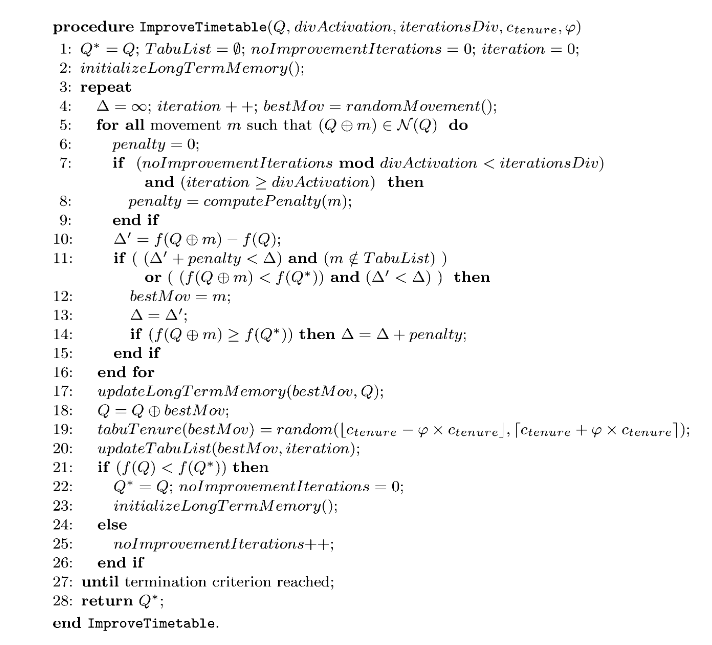
\includegraphics[width=1\textwidth]{./imagenes/CTTP.png}
    \caption{Pseudocódigo del algoritmo de búsqueda tabú para el CTTP \cite{tabuSearch}.}
    \label{fig:CTTP}
\end{figure}



\begin{landscape}
    

\begin{table}[h!]
    \centering
    \renewcommand{\arraystretch}{1.2}
    \begin{tabular}{|p{4cm}|p{4cm}|p{4cm}|p{4cm}|}
    \hline
    \textbf{Aspecto} & \textbf{Course Timetabling} & \textbf{Class/Teacher Timetabling} & \textbf{Examination Timetabling} \\ \hline
    
    \textbf{Objetivo Principal} & 
    Asignar horarios para cursos sin conflictos y equilibrar la carga semanal. & 
    Asignar horarios específicos a clases individuales y distribuir a los profesores eficientemente. & 
    Programar exámenes evitando conflictos y distribuyendo la carga de estudio. \\ \hline
    
    \textbf{Horizonte Temporal} & 
    Todo el semestre o año académico. & 
    Semanal durante el semestre o año académico. & 
    Periodo de exámenes, típicamente al final de un semestre. \\ \hline
    
    \textbf{Restricciones Clave} & 
    Disponibilidad de aulas, no superposición de cursos, balancear carga semanal de cursos. & 
    Disponibilidad de profesores y aulas, tamaño de clases, continuidad lógica de las clases. & 
    Evitar conflictos de horarios para estudiantes, minimizar exámenes consecutivos, disponibilidad de salas de examen. \\ \hline
    
    \textbf{Nivel de Abstracción} & 
    Macro: planificación de horarios generales para cursos completos. & 
    Micro: planificación de horarios detallados para clases y profesores. & 
    Específico: planificación de horarios de exámenes en un corto período. \\ \hline
    
    \textbf{Recursos Considerados} & 
    Aulas, disponibilidad de cursos. & 
    Aulas, disponibilidad de profesores, tamaño de clases. & 
    Salas de examen, supervisores, recursos específicos para exámenes. \\ \hline
    
    \textbf{Complejidad} & 
    Alta, pero menos que la programación de exámenes debido a un período más largo para distribuir cursos. & 
    Alta, con mayor detalle en la planificación respecto a profesores y clases. & 
    Muy alta, debido a la concentración de eventos en un corto período y la necesidad de evitar solapamientos. \\ \hline
    
    \end{tabular}
    \caption{Comparación entre Course Timetabling, Class/Teacher Timetabling y Examination Timetabling.}
    \label{tab:comparison}
    \end{table}
\end{landscape}

\section{Trabajos relacionados}

Para intentar solucionar el problema propuesto al principio del documento hay pocas alternativas existentes. Existen múltiples agendas y calendarios electrónicos que nos permitirían llevar el seguimiento de nuestro calendario semanal, pero no resuelven el problema (al menos de forma automática) de generar todas las combinaciones posibles para poder escoger la que más se adapte a nuestras necesidades.\newline

Voy a apoyarme en un caso práctico, para poder analizar las soluciones disponibles actualmente y poder evaluar el estado de la cuestión:\newline

Llega fin de curso, ya tenemos escogidas las asignaturas que planeamos cursar el próximo año y hemos recopilado de la información de los grupos y subgrupos de cada una de ellas. Sin embargo, las asignaturas se reparten entre 1º, 2º y 3º. Una de ellas necesitamos cursarla en un grupo concreto para convalidar las prácticas que tenemos aprobadas del curso pasado y a ser posible nos gustaría no pasar muchas horas al día en la facultad.

\subsection{Agendas y calendarios virtuales}
A priori la opción más simple y menos práctica. Organizamos los grupos según nuestras preferencias: rellenamos el calendario con el grupo del profesor que nos gustaría que nos convalidase las prácticas y vamos poco a poco, a base de en ensayo y error, introduciendo el resto de grupos y combinándolos para evitar solapamientos.

\subsection{Google Calendar}
Es un servicio de agenda y calendario en línea ofrecido por Google\footnote{\url{https://calendar.google.com/calendar}}.  Permite a los usuarios crear y editar eventos. Los eventos tienen una fecha y hora de inicio y fin, además de una descripción. Los usuarios pueden invitar a otros usuarios a sus eventos, y los eventos pueden ser públicos o privados. Los usuarios pueden ver sus eventos en una vista diaria, semanal o mensual. También permite a los usuarios generar múltiples calendarios y compartirlos con otros usuarios. Los usuarios pueden ver los calendarios de otras personas y superponerlos en su propio calendario. Google Calendar también se integra con otras aplicaciones de Google, como Gmail y Google Meet. Google Calendar también se integra con otras aplicaciones de calendario, como Microsoft Outlook y Apple Calendar. Está disponible en la web y en aplicaciones móviles para Android e iOS. Se muestra un ejemplo de uso en la Figura \ref{fig:google_calendar}.


\begin{figure}[H]
    \centering
    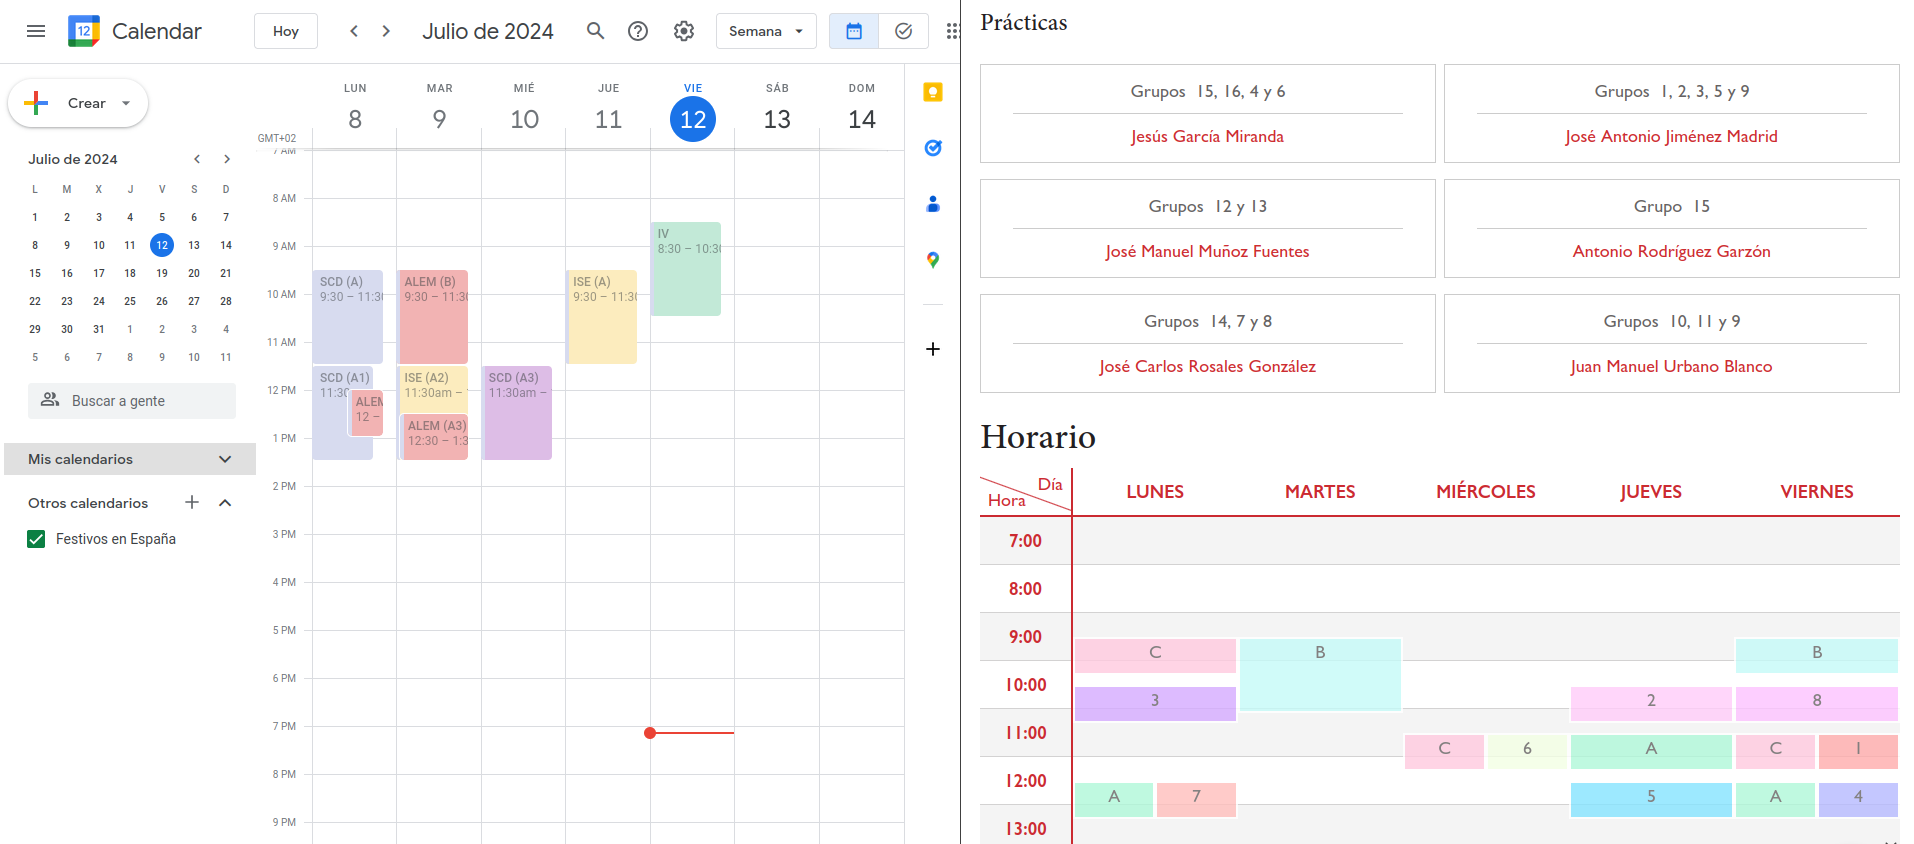
\includegraphics[width=1\textwidth]{./imagenes/Google_Calendar.png}
    \caption{Ejemplo de uso con Google Calendar.}
    \label{fig:google_calendar}
\end{figure}



\subsection{Microsoft Calendar}
Es una función integrada en aplicaciones como Outlook y Microsoft 365\footnote{\url{https://outlook.live.com/calendar}} que permite a los usuarios gestionar y organizar sus calendarios personales y profesionales. Facilita la creación y edición de citas, reuniones, y eventos, con opciones de recordatorios y notificaciones. Se sincroniza en la nube, ofreciendo acceso desde múltiples dispositivos, y permite compartir calendarios con otros usuarios. Además, se integra con otros servicios de calendario y herramientas de Microsoft, como Teams, facilitando la coordinación en equipos de trabajo y la gestión eficiente del tiempo. Se muestra un ejemplo de uso en la Figura \ref{fig:microsoft_calendar}.




\begin{figure}[H]
    \centering
    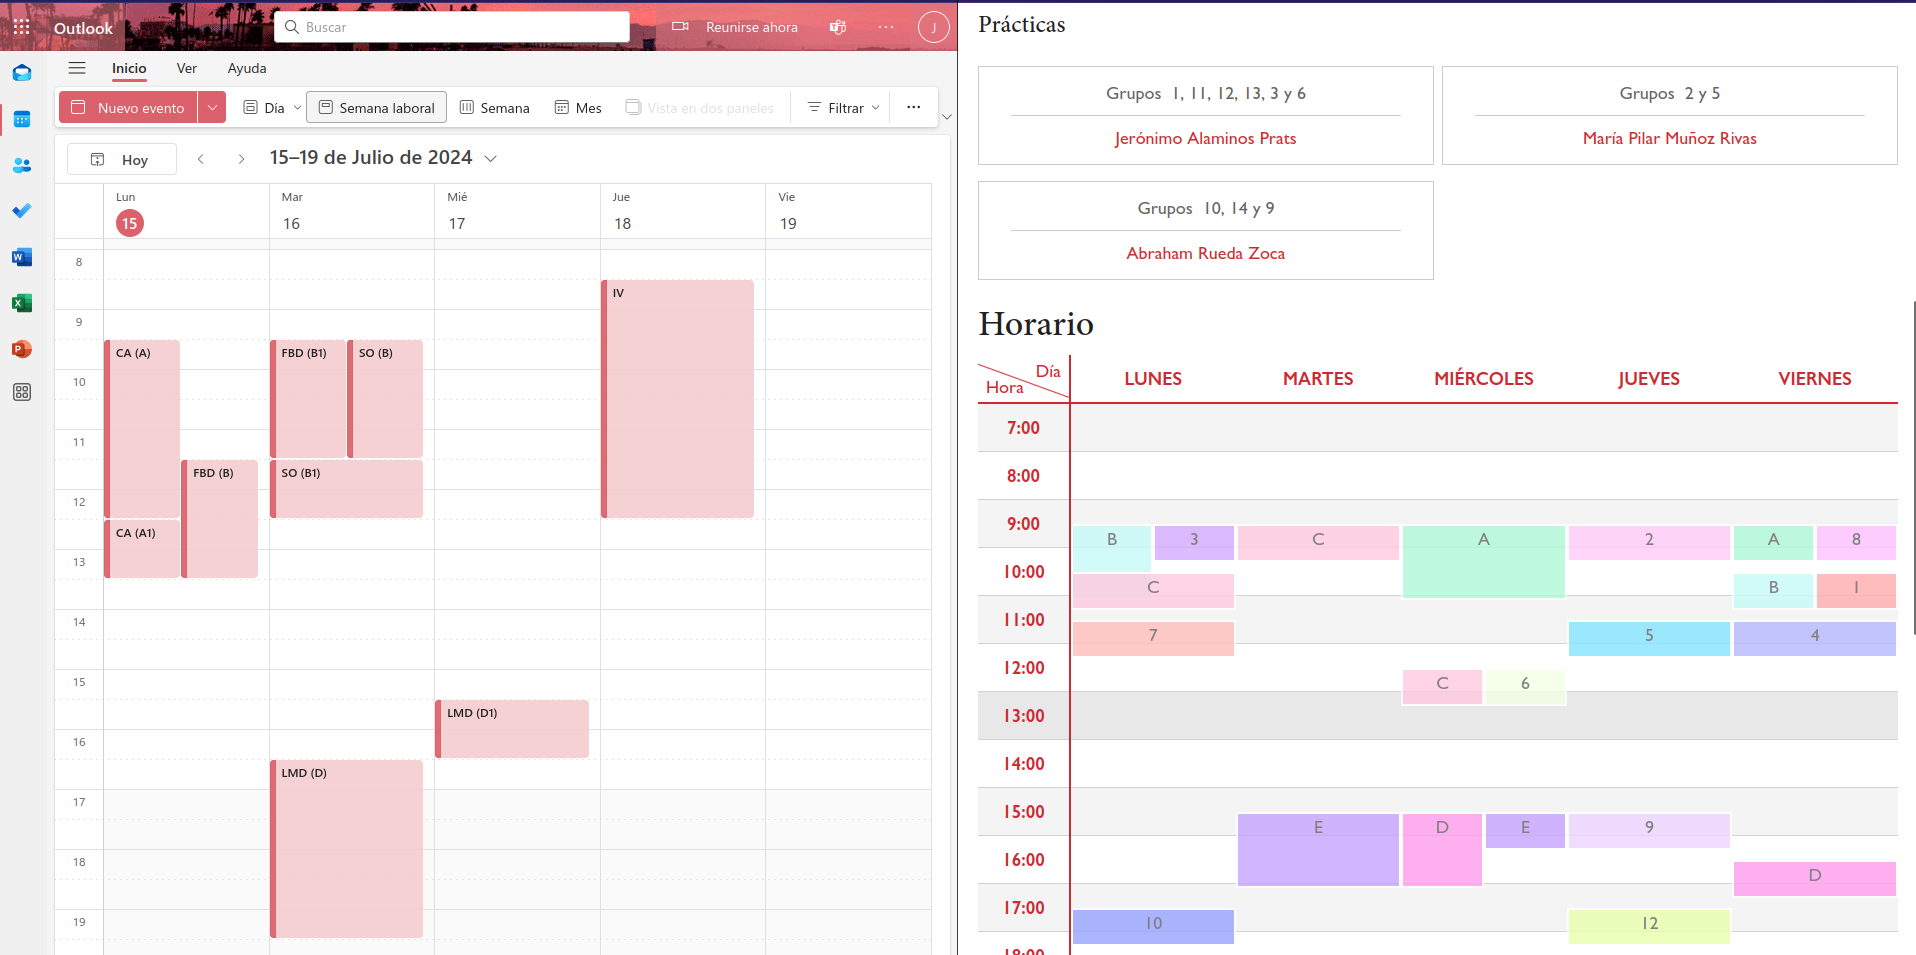
\includegraphics[width=1\textwidth]{./imagenes/Microsoft_calendar.png}
    \caption{Ejemplo de uso con Microsoft Calendar.}
    \label{fig:microsoft_calendar}
\end{figure}



\subsection{Proyectos académicos}

Además de las soluciones comerciales mencionadas, se encontró otro proyecto académico que aborda un enfoque similar al problema propuesto.

\begin{itemize}
    \item \textbf{Diego Barreiro Pérez}, \textit{Diseño e implementación de una aplicación web interactiva capaz de atender a preferencias y restricciones para la posterior generación automática de los horarios mediante heurísticas \cite{Barreiro}.}
\end{itemize}

% A continuación se muestran imágenes de los asistentes mencionados:\newpage
% \begin{figure}[ht!]
%     \begin{minipage}{1\linewidth}
%         \centering
%         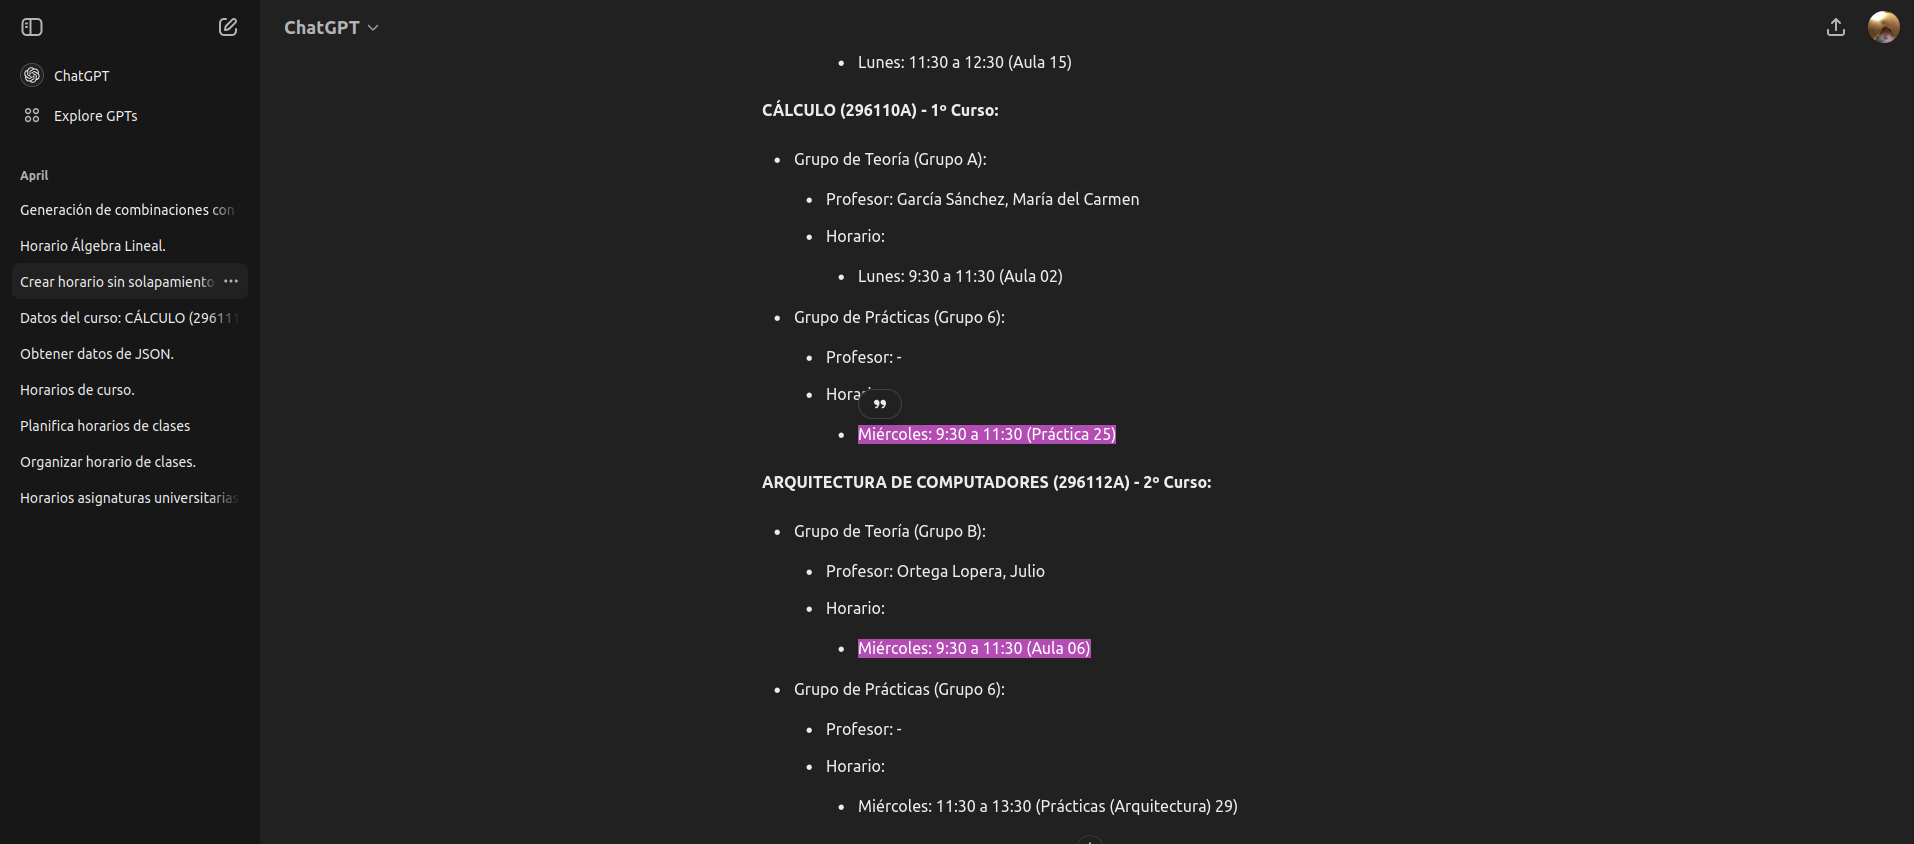
\includegraphics[width=\linewidth,height = 50mm]{./imagenes/ChatGPT.png}
%         \caption{Ejemplo con ChatGPT 3.5: solapa las clases.}
%         \vspace{0.5cm}
%     \end{minipage}
%     \begin{minipage}{1\linewidth}
%         \centering
%         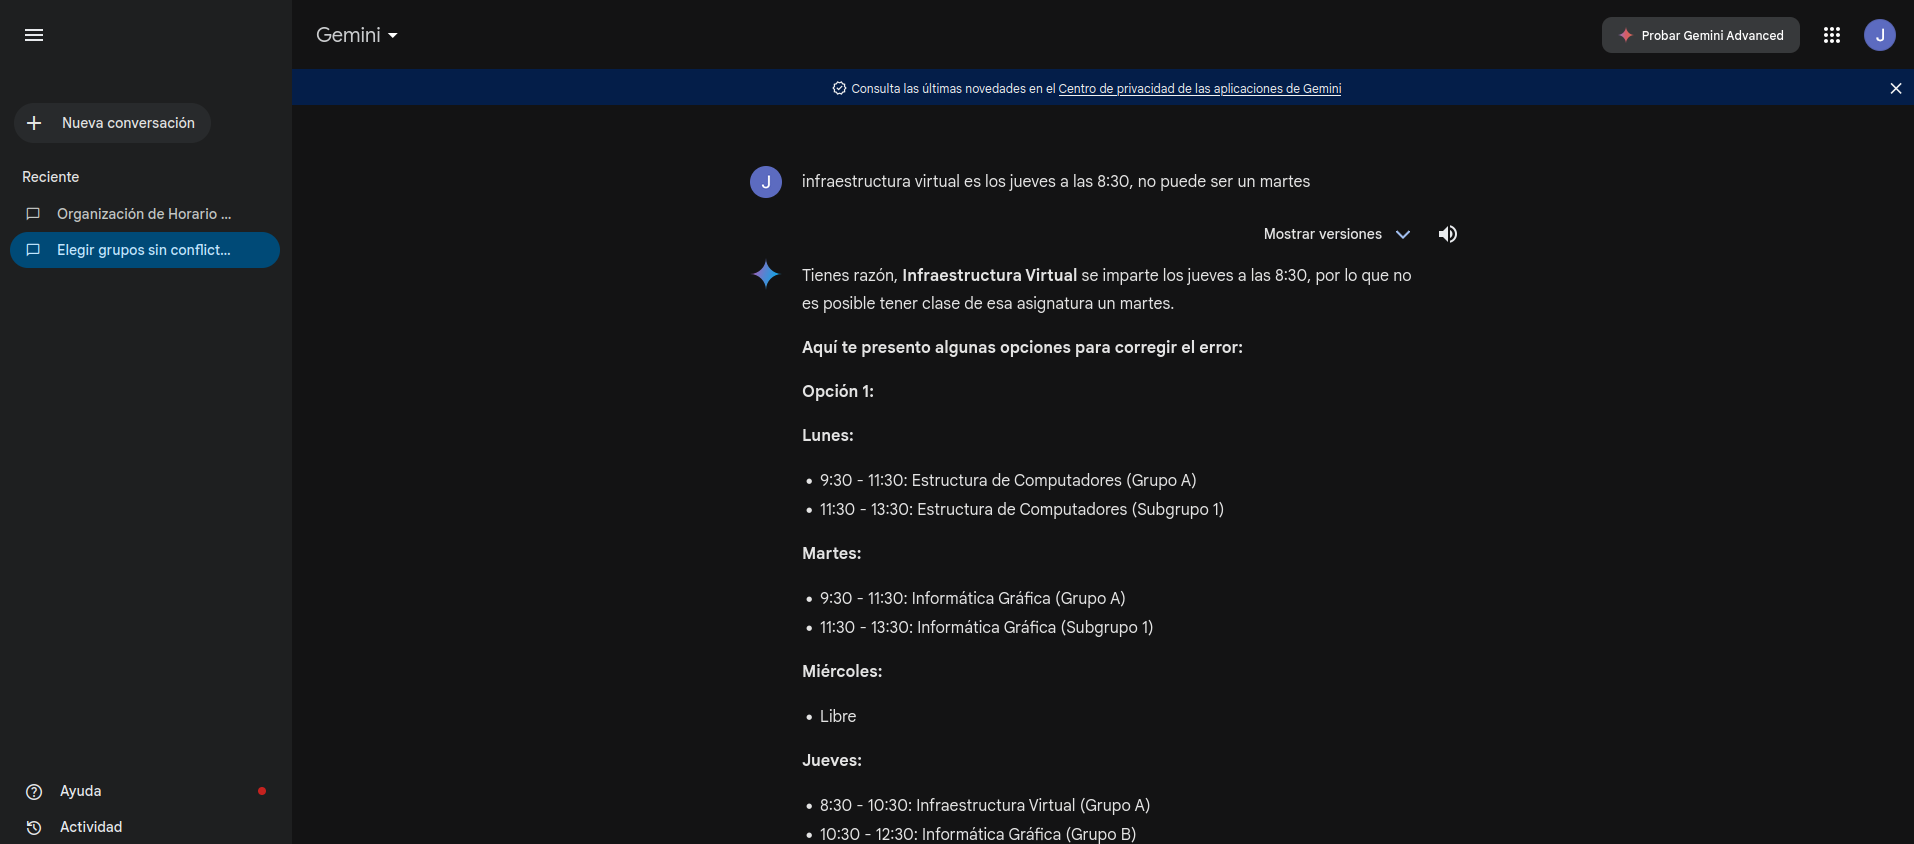
\includegraphics[width=\linewidth,height = 50mm]{./imagenes/Gemini.png}
%         \caption{Ejemplo con Gemini (Bard): omite asignaturas.}
%     \end{minipage}
% \end{figure}



% Existen múltiples estudios sobre algoritmos de timetabling para clases y exámenes universitarios:\\
\newpage
\subsection{Conclusiones}
Las aplicaciones discutidas anteriormente, como Google Calendar y Microsoft Calendar, son aplicaciones de calendario que permiten a los usuarios programar eventos y recordatorios. Se caracterizan por ser de propósito general, fáciles de usar y accesibles en múltiples dispositivos. Cuentan además con la ventaja de poder ser compartidos con otros usuarios, lo que facilita la colaboración en la programación de eventos.\newline

Por otro lado, los chatbots como ChatGPT y Gemini son aplicaciones de inteligencia artificial que permiten a los usuarios interactuar con un sistema de diálogo. Estos son capaces de responder preguntas y realizar tareas específicas. Son útiles para la programación de eventos en un calendario, ya que permiten a los usuarios interactuar con el sistema de forma natural y conversacional.\newline

Sin embargo, todas estas soluciones tienen una serie de limitaciones que las hacen inadecuadas para el problema propuesto. Entre ellas se incluyen:

\begin{enumerate}
    \item \textbf{Falta de automatización:} Los usuarios deben participar activamente en la organización de bloques para poder conformar el horario que se adecue a sus necesidades. Este proceso resulta ineficiente y tedioso.
    \item \textbf{Extracción de datos:} La información de los horarios de las asignaturas debe ser consultada e introducida manualmente por el usuario, lo que puede resultar en errores y omisiones.
\end{enumerate}

Respecto a los proyectos académicos, el propuesto por \textbf{Diego Barreiro Pérez}, pese a no contar con las limitaciones mencionadas anteriormente, resuelve un problema distinto al propuesto en este trabajo. Se trata de un algoritmo de timetabling del tipo UCTTP, por tanto se centra en la distribución de las clases en las franjas horarias y salas disponibles. En nuestro caso, dichos eventos ya están asignados y lo que se busca, es obtener la mejor combinación de los mismos para cumplir con las demandas del usuario concreto.\newline
	
	\chapter{Planificación}
\section{Presupuesto}

En esta sección se examinan y detallan los costos del proyecto. Se considerará el perfil de un ingeniero informático Junior, tomando en cuenta que el salario anual oscila entre los 20.000 € - 28.000 € \footnote{\url{https://www.glassdoor.es/Sueldos/junior-software-engineer-sueldo-SRCH_KO0,24.htm}}. Teniendo en cuenta que la implementación ha supuesto un aproximado de 200 horas. Partiendo de esta información, se puede calcular el coste total del salario del desarrollador, el cual se detalla a continuación:

\begin{equation}
    \textbf{Salario medio Ingeniero Junior} =  \frac {\text{24.000 €/Año} }{ \text{12 meses}} = \text{2.000 €/Mes}
\end{equation}

El salario por hora se calcula dividiendo el salario mensual entre 160 horas, que es el promedio de horas laborales al mes:

\begin{equation}
    \textbf{Salario por Hora} = \frac {\text{2.000 €/Mes}}{160 \text{ Horas}} = \text{12,50 €/Hora}
\end{equation}

Teniendo en cuenta las 200 horas de trabajo, se puede calcular el coste total del salario del desarrollador:

\begin{equation}
    \textbf{Coste Salario} = \text{200 Horas} \times \text{12,50 €/Hora} = \text{2.500 €}
\end{equation}

Para el diseño, se tendrá en cuenta el perfil de un diseñador gráfico, cuyo salario anual oscila entre los 17.000 € - 22.000 €. Teniendo en cuenta que el diseño ha supuesto un aproximado de 30 horas. Partiendo de esta información, se puede calcular el coste total del salario del diseñador, el cual se detalla a continuación:

\begin{equation}
    \textbf{Salario medio Diseñador Gráfico} =  \frac {\text{19.500 €/Año} }{ \text{12 meses}} = \text{1.625 €/Mes}
\end{equation}

El salario por hora se calcula dividiendo el salario mensual entre 160 horas, que es el promedio de horas laborales al mes:

\begin{equation}
    \textbf{Salario por Hora} = \frac {\text{1.625 €/Mes}}{160 \text{ Horas}} = \text{10,16 €/Hora}
\end{equation}

Teniendo en cuenta las 30 horas de trabajo, se puede calcular el coste total del salario del diseñador:

\begin{equation}
    \textbf{Coste Salario} = \text{30 Horas} \times \text{10,16 €/Hora} = \text{304,80 €}
\end{equation}

En cuanto a las licencias necesarias para este proyecto, se han utilizado exclusivamente tecnologías de código abierto con el propósito de reducir costos. Como resultado de esta decisión, no ha habido ningún gasto en licencias. Para calcular el coste del hardware mencionado en la sección de materiales, es esencial tener en cuenta la vida útil estimada de los dispositivos, como un portátil, que se estima en 5 años \footnote{\url{https://www.minitool.com/es/respaldar-datos/cuanto-dura-un-ordenador-portatil.html}}.

\begin{equation}
    \textbf{Coste Anual} = \frac {\text{Coste Materiales}}{\text{5 años}} = \text{169,38 €/año}
\end{equation}

\begin{equation}
    \textbf{Materiales x 8 Meses} = \left(\frac {\text{Coste Materiales}}{\text{5 años}}\right) \times 8 \text{ Meses} = \text{1.355,04 €}
\end{equation}

Sumando los costes de salario y materiales, se obtiene el coste total del proyecto (Figura \ref{tab:coste_total}).

\begin{table}[H]
    \centering
    \begin{tabular}{|c|c|ll}
    \cline{1-2}
    \multicolumn{1}{|l|}{Concepto} & \multicolumn{1}{l|}{Coste (€)} &  &  \\ \cline{1-2}
    Salario Desarrollador           & 2.500,00                        &  &  \\ \cline{1-2}
    Salario Diseñador               & 304,80                         &  &  \\ \cline{1-2}
    Materiales                      & 1.355,04                       &  &  \\ \cline{1-2}
    \textbf{Total}                   & \textbf{4.159,84}               &  &  \\ \cline{1-2}
    \end{tabular}
    \caption{Coste Total del Proyecto}
    \label{tab:coste_total}
\end{table}


	% Análisis del problema
	% 1. Análisis de requisitos
	% 2. Análisis de las soluciones
	% 3. Solucion propuesta
	% 4. Análisis de seguridad
	\chapter{Análisis}

En esta sección se cubren los requisitos funcionales y no funcionales para el desarrollo del proyecto. Se describen los casos de uso y se detallan los escenarios y actores del sistema.

\newpage
 
\section{Requisitos funcionales}

La calidad del software puede medirse en concordancia con los requisitos funcionales y de rendimiento que se establezcan, con las características intrínsecas que se esperan de cualquier software desarrollado de manera profesional. Los requisitos funcionales son aquellos que definen como debe comportarse el sistema, es decir, las funciones específicas que se esperan que cumplan con las necesidades finales del usuario \cite{Veloz_Segura_2022}.\newline

A continuación se describirán los requisitos funcionales, clasificados según su gestión principal, a fin de facilitar la comprensión clara de las funcionalidades que la plataforma debe incluir.

\subsection{Gestión de usuarios}

En este apartado se describen todas las funcionalidades relativas a los usuarios. Nótese que al referirnos al término ``usuario'' nos referimos a cualquier persona que haga uso de la plataforma, ya sea un administrador, un profesor o un alumno.
\newcounter{rfCounter}
\setcounter{rfCounter}{1}

\begin{table}[H]
    \centering
    \begin{tabular}{|p{4cm}|p{7cm}|}
    \hline
    \multicolumn{2}{|c|}{\textbf{RF\therfCounter\ - Registro de Usuario}} \\ \hline
    \textbf{Descripción} & Permite a un nuevo usuario registrarse en el sistema. \\ \hline
    \textbf{Datos de entrada} & Correo institucional. \\ \hline
    \textbf{Datos de salida} & Confirmación de registro. \\ \hline
    \end{tabular}
    \caption{RF\therfCounter\ - Registro de Usuario.}
    \stepcounter{rfCounter}
\end{table}

\begin{table}[H]
    \centering
    \begin{tabular}{|p{4cm}|p{7cm}|}
    \hline
    \multicolumn{2}{|c|}{\textbf{RF\therfCounter\ - Inicio de Sesión}} \\ \hline
    \textbf{Descripción} & Permite a un usuario identificarse y acceder a sus datos. \\ \hline
    \textbf{Datos de entrada} & Credenciales del usuario. \\ \hline
    \textbf{Datos de salida} & Avatar del usuario en la pantalla de inicio y acceso a la opción de consultar sus horarios. \\ \hline
    \end{tabular}
    \caption{RF\therfCounter\ - Inicio de Sesión.}
    \stepcounter{rfCounter}
\end{table}

\begin{table}[H]
    \centering
    \begin{tabular}{|p{4cm}|p{7cm}|}
    \hline
    \multicolumn{2}{|c|}{\textbf{RF\therfCounter\ - Baja de Usuario}} \\ \hline
    \textbf{Descripción} & Permite eliminar a un usuario del sistema y a sus datos asociados. \\ \hline
    \textbf{Datos de entrada} & Credenciales del usuario. \\ \hline
    \textbf{Datos de salida} & Confirmación de baja. \\ \hline
    \end{tabular}
    \caption{RF\therfCounter\ - Baja de Usuario.}
    \stepcounter{rfCounter}
\end{table}

\subsection{Gestión de Calendarios}

En este apartado se describe la gestión de los calendarios semanales creados por el usuario con el fin de organizar su matrícula o su horario de clases. Nótese que al referirnos al término ``combinación'' estamos haciendo referencia a uno de los calendarios semanales generados por el sistema con las asignaturas y grupos seleccionados por el usuario. 

\begin{table}[H]
    \centering
    \begin{tabular}{|p{4cm}|p{7cm}|}
    \hline
    \multicolumn{2}{|c|}{\textbf{RF\therfCounter\ - Seleccionar Grado}} \\ \hline
    \textbf{Descripción} & Permite al usuario seleccionar el grado de la UGR del que querrá organizar sus asignaturas. \\ \hline
    \textbf{Datos de entrada} & Lista de grados de la UGR. \\ \hline
    \textbf{Datos de salida} & Grado seleccionado. \\ \hline
    \end{tabular}
    \caption{RF\therfCounter\ - Seleccionar Grado.}
    \stepcounter{rfCounter}
\end{table}


\begin{table}[H]
    \centering
    \begin{tabular}{|p{4cm}|p{7cm}|}
    \hline
    \multicolumn{2}{|c|}{\textbf{RF\therfCounter\ - Seleccionar Curso}} \\ \hline
    \textbf{Descripción} & Permite al usuario seleccionar un curso académico. \\ \hline
    \textbf{Datos de entrada} & Lista de cursos del grado seleccionado. \\ \hline
    \textbf{Datos de salida} & Curso seleccionado. \\ \hline
    \end{tabular}
    \caption{RF\therfCounter\ - Seleccionar Curso.}
    \stepcounter{rfCounter}
\end{table}

\begin{table}[H]
    \centering
    \begin{tabular}{|p{4cm}|p{7cm}|}
    \hline
    \multicolumn{2}{|c|}{\textbf{RF\therfCounter\ - Seleccionar Cuatrimestre}} \\ \hline
    \textbf{Descripción} & Permite al usuario seleccionar un cuatrimestre del curso académico seleccionado. \\ \hline
    \textbf{Datos de entrada} & Lista de cuatrimestres del curso y grado seleccionado. \\ \hline
    \textbf{Datos de salida} & Cuatrimestre seleccionado. \\ \hline
    \end{tabular}
    \caption{RF\therfCounter\ - Seleccionar Cuatrimestre.}
    \stepcounter{rfCounter}
\end{table}

\begin{table}[H]
    \centering
    \begin{tabular}{|p{4cm}|p{7cm}|}
    \hline
    \multicolumn{2}{|c|}{\textbf{RF\therfCounter\ - Seleccionar Asignatura}} \\ \hline
    \textbf{Descripción} & Permite al usuario seleccionar una asignatura para incluirla en la planificación de su calendario semanal. \\ \hline
    \textbf{Datos de entrada} & Lista de asignaturas del grado seleccionado. \\ \hline
    \textbf{Datos de salida} & Asignatura seleccionada. \\ \hline
    \end{tabular}
    \caption{RF\therfCounter\ - Seleccionar Asignatura.}
    \stepcounter{rfCounter}
\end{table}

\begin{table}[H]
    \centering
    \begin{tabular}{|p{4cm}|p{7cm}|}
    \hline
    \multicolumn{2}{|c|}{\textbf{RF\therfCounter\ - Seleccionar Grupo}} \\ \hline
    \textbf{Descripción} & Permite al usuario seleccionar un grupo de teoría a planificar para la asignatura que ha previamente seleccionado. \\ \hline
    \textbf{Datos de entrada} & Lista de grupos de la asignatura seleccionada. \\ \hline
    \textbf{Datos de salida} & Grupo seleccionado. \\ \hline
    \end{tabular}
    \caption{RF\therfCounter\ - Seleccionar Grupo.}
    \stepcounter{rfCounter}
\end{table}

\begin{table}[H]
    \centering
    \begin{tabular}{|p{4cm}|p{7cm}|}
    \hline
    \multicolumn{2}{|c|}{\textbf{RF\therfCounter\ - Seleccionar Combinación}} \\ \hline
    \textbf{Descripción} & Permite al usuario seleccionar una combinación de las generadas por el sistema con su selección de asignaturas y grupos. \\ \hline
    \textbf{Datos de entrada} & Lista de combinaciones generadas. \\ \hline
    \textbf{Datos de salida} & Combinación seleccionada. \\ \hline
    \end{tabular}
    \caption{RF\therfCounter\ - Seleccionar Calendario.}
    \stepcounter{rfCounter}
\end{table}

\begin{table}[H]
    \centering
    \begin{tabular}{|p{4cm}|p{7cm}|}
    \hline
    \multicolumn{2}{|c|}{\textbf{RF\therfCounter\ - Descargar Combinación}} \\ \hline
    \textbf{Descripción} & Permite al usuario descargar la combinación deseada en formato PDF. \\ \hline
    \textbf{Datos de entrada} & Combinación seleccionada. \\ \hline
    \textbf{Datos de salida} & Calendario de la combinación seleccionada en formato PDF. \\ \hline
    \end{tabular}
    \caption{RF\therfCounter\ - Descargar Combinación.}
    \stepcounter{rfCounter}
\end{table}

\begin{table}[H]
    \centering
    \begin{tabular}{|p{4cm}|p{7cm}|}
    \hline
    \multicolumn{2}{|c|}{\textbf{RF\therfCounter\ - Guardar Calendario}} \\ \hline
    \textbf{Descripción} & Permite al usuario guardar la combinación seleccionada en el sistema para consultarla posteriormente. \\ \hline
    \textbf{Datos de entrada} & Combinación seleccionada. \\ \hline
    \textbf{Datos de salida} & Combinación guardada como calendario. \\ \hline
    \end{tabular}
    \caption{RF\therfCounter\ - Guardar Calendario.}
    \stepcounter{rfCounter}
\end{table}

\begin{table}[H]
    \centering
    \begin{tabular}{|p{4cm}|p{7cm}|}
    \hline
    \multicolumn{2}{|c|}{\textbf{RF\therfCounter\ - Consultar Calendario}} \\ \hline
    \textbf{Descripción} & Permite al usuario consultar sus calendarios finales guardados. \\ \hline
    \textbf{Datos de entrada} & Lista de calendarios guardados. \\ \hline
    \textbf{Datos de salida} & Calendario guardado seleccionado. \\ \hline
    \end{tabular}
    \caption{RF\therfCounter\ - Consultar Calendario.}
    \stepcounter{rfCounter}
\end{table}

\section{Requisitos no funcionales}

Los requisitos no funcionales son aquellos que no se refieren específicamente a la funcionalidad de un sistema. Imponen restricciones sobre el producto que se está desarrollando y el proceso de desarrollo, y especifican restricciones externas que debe cumplir el producto \cite{nonFR}.

\newcounter{nrfCounter}
\setcounter{nrfCounter}{1}

\begin{table}[H]
    \centering
    \begin{tabular}{|p{4cm}|p{7cm}|}
    \hline
    \multicolumn{2}{|c|}{\textbf{RNF\thenrfCounter\ - Usabilidad}} \\ \hline
    \textbf{Descripción} & La plataforma debe ser fácil e intuitiva para los usuarios. \\ \hline
    \textbf{Criterios} & Interfaz de usuario sencilla y autoexplicativa. \\ \hline
    \end{tabular}
    \caption{RNF\thenrfCounter\ - Usabilidad.}
    \stepcounter{nrfCounter}
\end{table}

\begin{table}[H]
    \centering
    \begin{tabular}{|p{4cm}|p{7cm}|}
    \hline
    \multicolumn{2}{|c|}{\textbf{RNF\thenrfCounter\ - Rendimiento}} \\ \hline
    \textbf{Descripción} & La plataforma debe responder con rapidez a las consultas del usuario. \\ \hline
    \textbf{Criterios} & Tiempos de respuesta rápidos para las peticiones. \\ \hline
    \end{tabular}
    \caption{RNF\thenrfCounter\ - Rendimiento.}
    \stepcounter{nrfCounter}
\end{table}

\begin{table}[H]
    \centering
    \begin{tabular}{|p{4cm}|p{7cm}|}
    \hline
    \multicolumn{2}{|c|}{\textbf{RNF\thenrfCounter\ - Eficiencia}} \\ \hline
    \textbf{Descripción} & La plataforma debe reducir el tiempo que el usuario tardaría en hacer su calendario semanal manualmente. \\ \hline
    \textbf{Criterios} & Proceso rápido y automático de generación del calendario. \\ \hline
    \end{tabular}
    \caption{RNF\thenrfCounter\ - Eficiencia.}
    \stepcounter{nrfCounter}
\end{table}

\begin{table}[H]
    \centering
    \begin{tabular}{|p{4cm}|p{7cm}|}
    \hline
    \multicolumn{2}{|c|}{\textbf{RNF\thenrfCounter\ - Compatibilidad}} \\ \hline
    \textbf{Descripción} & La plataforma funcionará correctamente independientemente del navegador o dispositivo usado. \\ \hline
    \textbf{Criterios} & React permite un diseño responsive y React Native permite desplegar archivos APK para Android y archivos para iOS  . \\ \hline
    \end{tabular}
    \caption{RNF\thenrfCounter\ - Compatibilidad.}
    \stepcounter{nrfCounter}
\end{table}

\begin{table}[H]
    \centering
    \begin{tabular}{|p{4cm}|p{7cm}|}
    \hline
    \multicolumn{2}{|c|}{\textbf{RNF\thenrfCounter\ - Mantenibilidad}} \\ \hline
    \textbf{Descripción} & La plataforma facilitará las actualizaciones y el desarrollo de su contenido. \\ \hline
    \textbf{Criterios} & La documentación y el código de la plataforma se desarrollarán de forma clara para facilitar su entendimiento y posterior actualización. \\ \hline
    \end{tabular}
    \caption{RNF\thenrfCounter\ - Mantenibilidad.}
    \stepcounter{nrfCounter}
\end{table}

\section{Modelo de Caso de Uso}

Los casos de uso son una secuencia de eventos que en conjunto, conducen a un sistema haciendo algo útil. Describen las diferentes formas en que los usuarios interaccionan con el mismo y como este les responde. Son una herramienta fundamental para la comprensión de los requisitos funcionales y ayudan a entender las funcionalidades esperadas del sistema y las partes implicadas \cite{bittner2003use}.

\subsection{Actores del Sistema}

La interacción con la plataforma se basa en dos tipos de actores: los usuarios sin registrar y los usuarios registrados. El acceso no está restringido a usuarios registrados, pero estos últimos disponen de funcionalidades adicionales.

\begin{enumerate}
    \item \textbf{Usuario genérico}: Son los usuarios que acceden a la plataforma para generar sus calendarios semanales y es principalmente a quien va dirigida la plataforma. Pueden seleccionar el grado, curso, cuatrimestre, asignaturas y grupos que desean incluir en su calendario semanal. Consultar los calendarios generados, descargarlos en formato PDF y guardarlos en la plataforma para consultarlos posteriormente.
    \item \textbf{Usuario Registrado}: Son los usuarios que han completado el proceso de registro en la plataforma. Tienen acceso a las mismas funcionalidades que los usuarios genéricos, pero además pueden guardar sus calendarios semanales en la plataforma para consultarlos posteriormente.
\end{enumerate}

\subsection{Escenarios de Casos de Uso}

\newcounter{ccCounter}
\setcounter{ccCounter}{1}
% Ajustar el espacio entre elementos flotantes
\setlength{\textfloatsep}{5pt plus 1.0pt minus 2.0pt} % Espacio entre el texto y los elementos flotantes
\setlength{\floatsep}{5pt plus 1.0pt minus 2.0pt} % Espacio entre dos elementos flotantes
\setlength{\intextsep}{5pt plus 1.0pt minus 2.0pt} % Espacio entre el texto y los elementos flotantes insertados en el texto


\begin{table}[H]
    \centering
    \begin{tabular}{|p{4cm}|p{7cm}|}
    \hline
    \multicolumn{2}{|c|}{\textbf{CU\theccCounter\ - Registrar Usuario}} \\ \hline
    \textbf{Actores} & Usuario Genérico. \\ \hline
    \textbf{Precondiciones} & El actor no está registrado en el sistema. \\ \hline
    \textbf{Postcondiciones} & El actor está registrado en el sistema. \\ \hline
    \textbf{Flujo principal} & \begin{minipage}[t]{\linewidth}
        \vspace{1pt}
        \begin{enumerate}
            \setlength{\itemsep}{0pt}
            \setlength{\parskip}{0pt}
            \setlength{\parsep}{0pt}
            \item El actor accede a la plataforma.
            \item El actor ingresa su correo institucional.
            \item El sistema envía un correo de confirmación al correo institucional del actor.
            \item El actor confirma su registro en la plataforma.
            \item El sistema registra al actor en la plataforma.
        \end{enumerate}
        \vspace{1pt}
    \end{minipage} \\ \hline  
    \end{tabular}
    \caption{CU\theccCounter\ - Registrar Usuario.}
    \stepcounter{ccCounter}
\end{table}

\begin{table}[H]
    \centering
    \begin{tabular}{|p{4cm}|p{7cm}|}
    \hline
    \multicolumn{2}{|c|}{\textbf{CU\theccCounter\ - Autenticar Usuario}} \\ \hline
    \textbf{Actores} & Usuario Registrado. \\ \hline
    \textbf{Precondiciones} & El actor está registrado en el sistema. \\ \hline
    \textbf{Postcondiciones} & El actor está autenticado en el sistema. \\ \hline
    \textbf{Flujo principal} & \begin{minipage}[t]{\linewidth}
        \vspace{1pt}
        \begin{enumerate}
            \setlength{\itemsep}{0pt}
            \setlength{\parskip}{0pt}
            \setlength{\parsep}{0pt}
            \item El actor accede a la plataforma.
            \item El actor ingresa sus credenciales.
            \item El sistema valida sus credenciales.
            \item El sistema muestra el avatar del actor en la pantalla de inicio y le da acceso a la opción de consultar sus horarios.
        \end{enumerate}
        \vspace{1pt}
    \end{minipage} \\ \hline  
    \end{tabular}
    \caption{CU\theccCounter\ - Autenticar Usuario.}
    \stepcounter{ccCounter}
\end{table}

\begin{table}[H]
    \centering
    \begin{tabular}{|p{4cm}|p{7cm}|}
    \hline
    \multicolumn{2}{|c|}{\textbf{CU\theccCounter\ - Eliminar Usuario}} \\ \hline
    \textbf{Actores} & Usuario Registrado. \\ \hline
    \textbf{Precondiciones} & El actor está registrado en el sistema. \\ \hline
    \textbf{Postcondiciones} & El actor no está registrado en el sistema. \\ \hline
    \textbf{Flujo principal} & \begin{minipage}[t]{\linewidth}
        \vspace{1pt}
        \begin{enumerate}
            \setlength{\itemsep}{0pt}
            \setlength{\parskip}{0pt}
            \setlength{\parsep}{0pt}
            \item El actor accede a la plataforma.
            \item El actor selecciona la opción de eliminar su cuenta.
            \item El sistema solicita confirmación al actor.
            \item El actor confirma la eliminación de su cuenta.
            \item El sistema elimina al actor de la plataforma y sus datos asociados.
        \end{enumerate}
        \vspace{1pt}
    \end{minipage} \\ \hline  
    \end{tabular}
    \caption{CU\theccCounter\ - Eliminar Usuario.}
    \stepcounter{ccCounter}
\end{table}

\begin{table}[H]
    \centering
    \begin{tabular}{|p{4cm}|p{7cm}|}
    \hline
    \multicolumn{2}{|c|}{\textbf{CU\theccCounter\ - Seleccionar Grado}} \\ \hline
    \textbf{Actores} & Usuario Genérico y Usuario Registrado. \\ \hline
    \textbf{Precondiciones} & El actor accede a la plataforma. \\ \hline
    \textbf{Postcondiciones} & Se muestran los datos del grado seleccionado. \\ \hline
    \textbf{Flujo principal} & \begin{minipage}[t]{\linewidth}
        \vspace{1pt}
        \begin{enumerate}
            \setlength{\itemsep}{0pt}
            \setlength{\parskip}{0pt}
            \setlength{\parsep}{0pt}
            \item El actor accede a la plataforma.
            \item El sistema muestra la lista de grados disponibles.
            \item El actor selecciona el grado de interés.
            \item El sistema muestra los datos del grado seleccionado.
        \end{enumerate}
        \vspace{1pt}
    \end{minipage} \\ \hline  
    \end{tabular}
    \caption{CU\theccCounter\ - Seleccionar Grado.}
    \stepcounter{ccCounter}
\end{table}

\begin{table}[H]
    \centering
    \begin{tabular}{|p{4cm}|p{7cm}|}
    \hline
    \multicolumn{2}{|c|}{\textbf{CU\theccCounter\ - Seleccionar Curso}} \\ \hline
    \textbf{Actores} & Usuario Genérico y Usuario Registrado. \\ \hline
    \textbf{Precondiciones} & El actor accede a la plataforma. \\ \hline
    \textbf{Postcondiciones} & Se muestran los datos del curso seleccionado. \\ \hline
    \textbf{Flujo principal} & \begin{minipage}[t]{\linewidth}
        \vspace{1pt}
        \begin{enumerate}
            \setlength{\itemsep}{0pt}
            \setlength{\parskip}{0pt}
            \setlength{\parsep}{0pt}
            \item El actor accede a la plataforma.
            \item El sistema muestra la lista de grados disponibles.
            \item El actor selecciona el grado de interés.
            \item El sistema muestra la lista de cursos disponibles.
            \item El actor selecciona el curso de interés.
            \item El sistema muestra los datos del curso seleccionado.
        \end{enumerate}
        \vspace{1pt}
    \end{minipage} \\ \hline  
    \end{tabular}
    \caption{CU\theccCounter\ - Seleccionar Curso.}
    \stepcounter{ccCounter}
\end{table}

\begin{table}[H]
    \centering
    \begin{tabular}{|p{4cm}|p{7cm}|}
    \hline
    \multicolumn{2}{|c|}{\textbf{CU\theccCounter\ - Seleccionar Cuatrimestre}} \\ \hline
    \textbf{Actores} & Usuario Genérico y Usuario Registrado. \\ \hline
    \textbf{Precondiciones} & El actor accede a la plataforma. \\ \hline
    \textbf{Postcondiciones} & Se muestran los datos del cuatrimestre seleccionado. \\ \hline
    \textbf{Flujo principal} & \begin{minipage}[t]{\linewidth}
        \vspace{1pt}
        \begin{enumerate}
            \setlength{\itemsep}{0pt}
            \setlength{\parskip}{0pt}
            \setlength{\parsep}{0pt}
            \item El actor accede a la plataforma.
            \item El sistema muestra la lista de grados disponibles.
            \item El actor selecciona el grado de interés.
            \item El sistema muestra los datos del grado seleccionado.
            \item El actor selecciona el curso académico de interés.
            \item El sistema muestra la lista de cuatrimestres disponibles.
            \item El actor selecciona el cuatrimestre de interés.
            \item El sistema muestra los datos del cuatrimestre seleccionado.
        \end{enumerate}
        \vspace{1pt}
    \end{minipage} \\ \hline  
    \end{tabular}
    \caption{CU\theccCounter\ - Seleccionar Cuatrimestre.}
    \stepcounter{ccCounter}
\end{table}

\begin{table}[H]
    \centering
    \begin{tabular}{|p{4cm}|p{7cm}|}
    \hline
    \multicolumn{2}{|c|}{\textbf{CU\theccCounter\ - Seleccionar Asignaturas}} \\ \hline
    \textbf{Actores} & Usuario Genérico y Usuario Registrado. \\ \hline
    \textbf{Precondiciones} & El actor accede a la plataforma. \\ \hline
    \textbf{Postcondiciones} & Se muestra la selección de asignaturas hecha por el actor. \\ \hline
    \textbf{Flujo principal} & \begin{minipage}[t]{\linewidth}
        \vspace{1pt}
        \begin{enumerate}
            \setlength{\itemsep}{0pt}
            \setlength{\parskip}{0pt}
            \setlength{\parsep}{0pt}
            \item El actor accede a la plataforma.
            \item El sistema muestra la lista de grados disponibles.
            \item El actor selecciona el grado de interés.
            \item El sistema muestra los datos del grado seleccionado.
            \item El actor selecciona el curso académico de interés.
            \item El actor selecciona el cuatrimestre de interés.
            \item El actor selecciona la asignatura de interés.
        \end{enumerate}
        \vspace{1pt}
    \end{minipage} \\ \hline  
    \end{tabular}
    \caption{CU\theccCounter\ - Seleccionar Asignaturas.}
    \stepcounter{ccCounter}
\end{table}

\begin{table}[H]
    \centering
    \begin{tabular}{|p{4cm}|p{7cm}|}
    \hline
    \multicolumn{2}{|c|}{\textbf{CU\theccCounter\ - Seleccionar Grupos}} \\ \hline
    \textbf{Actores} & Usuario Genérico y Usuario Registrado. \\ \hline
    \textbf{Precondiciones} & El actor accede a la plataforma. \\ \hline
    \textbf{Postcondiciones} & Se muestra la lista de grupos de la selección de asignaturas hecha por el actor. \\ \hline
    \textbf{Flujo principal} & \begin{minipage}[t]{\linewidth}
        \vspace{1pt}
        \begin{enumerate}
            \setlength{\itemsep}{0pt}
            \setlength{\parskip}{0pt}
            \setlength{\parsep}{0pt}
            \item El actor accede a la plataforma.
            \item El sistema muestra la lista de grados disponibles.
            \item El actor selecciona el grado de interés.
            \item El sistema muestra los datos del grado seleccionado.
            \item El actor selecciona el curso académico de interés.
            \item El actor selecciona el cuatrimestre de interés.
            \item El actor selecciona la asignatura de interés.
            \item El actor selecciona el grupo de interés.
        \end{enumerate}
        \vspace{1pt}
    \end{minipage} \\ \hline  
    \end{tabular}
    \caption{CU\theccCounter\ - Seleccionar Grupos.}
    \stepcounter{ccCounter}
\end{table}

\begin{table}[H]
    \centering
    \begin{tabular}{|p{4cm}|p{7cm}|}
    \hline
    \multicolumn{2}{|c|}{\textbf{CU\theccCounter\ - Seleccionar Combinación}} \\ \hline
    \textbf{Actores} & Usuario Genérico y Usuario Registrado. \\ \hline
    \textbf{Precondiciones} & El actor accede a la plataforma. \\ \hline
    \textbf{Postcondiciones} & Se muestra la lista de combinaciones de grupos de la selección de asignaturas y grupos hecha por el actor. \\ \hline
    \textbf{Flujo principal} & \begin{minipage}[t]{\linewidth}
        \vspace{1pt}
        \begin{enumerate}
            \setlength{\itemsep}{0pt}
            \setlength{\parskip}{0pt}
            \setlength{\parsep}{0pt}
            \item El actor accede a la plataforma.
            \item El sistema muestra la lista de grados disponibles.
            \item El actor selecciona el grado de interés.
            \item El sistema muestra los datos del grado seleccionado.
            \item El actor selecciona el curso académico de interés.
            \item El actor selecciona el cuatrimestre de interés.
            \item El actor selecciona la asignatura de interés.
            \item El actor selecciona el grupo de interés.
            \item El actor selecciona la combinación de interés.
        \end{enumerate}
        \vspace{1pt}
    \end{minipage} \\ \hline  
    \end{tabular}
    \caption{CU\theccCounter\ - Seleccionar Combinación.}
    \stepcounter{ccCounter}
\end{table}

\begin{table}[H]
    \centering
    \begin{tabular}{|p{4cm}|p{7cm}|}
    \hline
    \multicolumn{2}{|c|}{\textbf{CU\theccCounter\ - Guardar Combinación}} \\ \hline
    \textbf{Actores} & Usuario Registrado. \\ \hline
    \textbf{Precondiciones} & El actor debe estar registrado en la plataforma. \\ \hline
    \textbf{Postcondiciones} & Se guarda la combinación selecciona. \\ \hline
    \textbf{Flujo principal} & \begin{minipage}[t]{\linewidth}
        \vspace{1pt}
        \begin{enumerate}
            \setlength{\itemsep}{0pt}
            \setlength{\parskip}{0pt}
            \setlength{\parsep}{0pt}
            \item El actor accede a la plataforma.
            \item El sistema muestra la lista de grados disponibles.
            \item El actor selecciona el grado de interés.
            \item El sistema muestra los datos del grado seleccionado.
            \item El actor selecciona el curso académico de interés.
            \item El actor selecciona el cuatrimestre de interés.
            \item El actor selecciona la asignatura de interés.
            \item El actor selecciona el grupo de interés.
            \item El actor selecciona la combinación de interés.
            \item El actor selecciona la opción de guardar la combinación.
        \end{enumerate}
        \vspace{1pt}
    \end{minipage} \\ \hline  
    \end{tabular}
    \caption{CU\theccCounter\ - Guardar Combinación.}
    \stepcounter{ccCounter}
\end{table}

\begin{table}[H]
    \centering
    \begin{tabular}{|p{4cm}|p{7cm}|}
    \hline
    \multicolumn{2}{|c|}{\textbf{CU\theccCounter\ - Consultar Horarios Almacenados}} \\ \hline
    \textbf{Actores} & Usuario Registrado. \\ \hline
    \textbf{Precondiciones} & El actor está registrado, autenticado en el sistema y ha guardado algún calendario. \\ \hline
    \textbf{Postcondiciones} & Se muestran los calendarios del actor. \\ \hline
    \textbf{Flujo principal} & \begin{minipage}[t]{\linewidth}
        \vspace{1pt}
        \begin{enumerate}
            \setlength{\itemsep}{0pt}
            \setlength{\parskip}{0pt}
            \setlength{\parsep}{0pt}
            \item El actor accede a la plataforma.
            \item El actor ingresa sus crendenciales.
            \item El sistema autentifica al usuario.
            \item El actor selecciona la opción ``Consultar Mis Horarios''.
            \item El sistema muestra sus calendarios guardados.
        \end{enumerate}
        \vspace{1pt}
    \end{minipage} \\ \hline  
    \end{tabular}
    \caption{CU\theccCounter\ - Consultar Horarios Almacenados.}
    \stepcounter{ccCounter}
\end{table}


\begin{table}[H]
    \centering
    \begin{tabular}{|p{4cm}|p{7cm}|}
    \hline
    \multicolumn{2}{|c|}{\textbf{CU\theccCounter\ - Descargar Combinación}} \\ \hline
    \textbf{Actores} & Usuario Genérico y Usuario Registrado. \\ \hline
    \textbf{Precondiciones} & El actor accede a la plataforma. \\ \hline
    \textbf{Postcondiciones} & Se guarda la combinación selecciona. \\ \hline
    \textbf{Flujo principal} & \begin{minipage}[t]{\linewidth}
        \vspace{1pt}
        \begin{enumerate}
            \setlength{\itemsep}{0pt}
            \setlength{\parskip}{0pt}
            \setlength{\parsep}{0pt}
            \item El actor accede a la plataforma.
            \item El sistema muestra la lista de grados disponibles.
            \item El actor selecciona el grado de interés.
            \item El sistema muestra los datos del grado seleccionado.
            \item El actor selecciona el curso académico de interés.
            \item El actor selecciona el cuatrimestre de interés.
            \item El actor selecciona la asignatura de interés.
            \item El actor selecciona el grupo de interés.
            \item El actor selecciona la combinación de interés.
            \item El actor selecciona la opción de descargar la combinación.
        \end{enumerate}
        \vspace{1pt}
    \end{minipage} \\ \hline  
    \end{tabular}
    \caption{CU\theccCounter\ - Descargar Combinación.}
    \stepcounter{ccCounter}
\end{table}

A continuación un diagrama de casos de uso con actores comunes en la Figura \ref{fig:CC_Actores_Comunes}.

\vspace{2pt}
\begin{landscape}
    \begin{figure}[H]
        \centering
        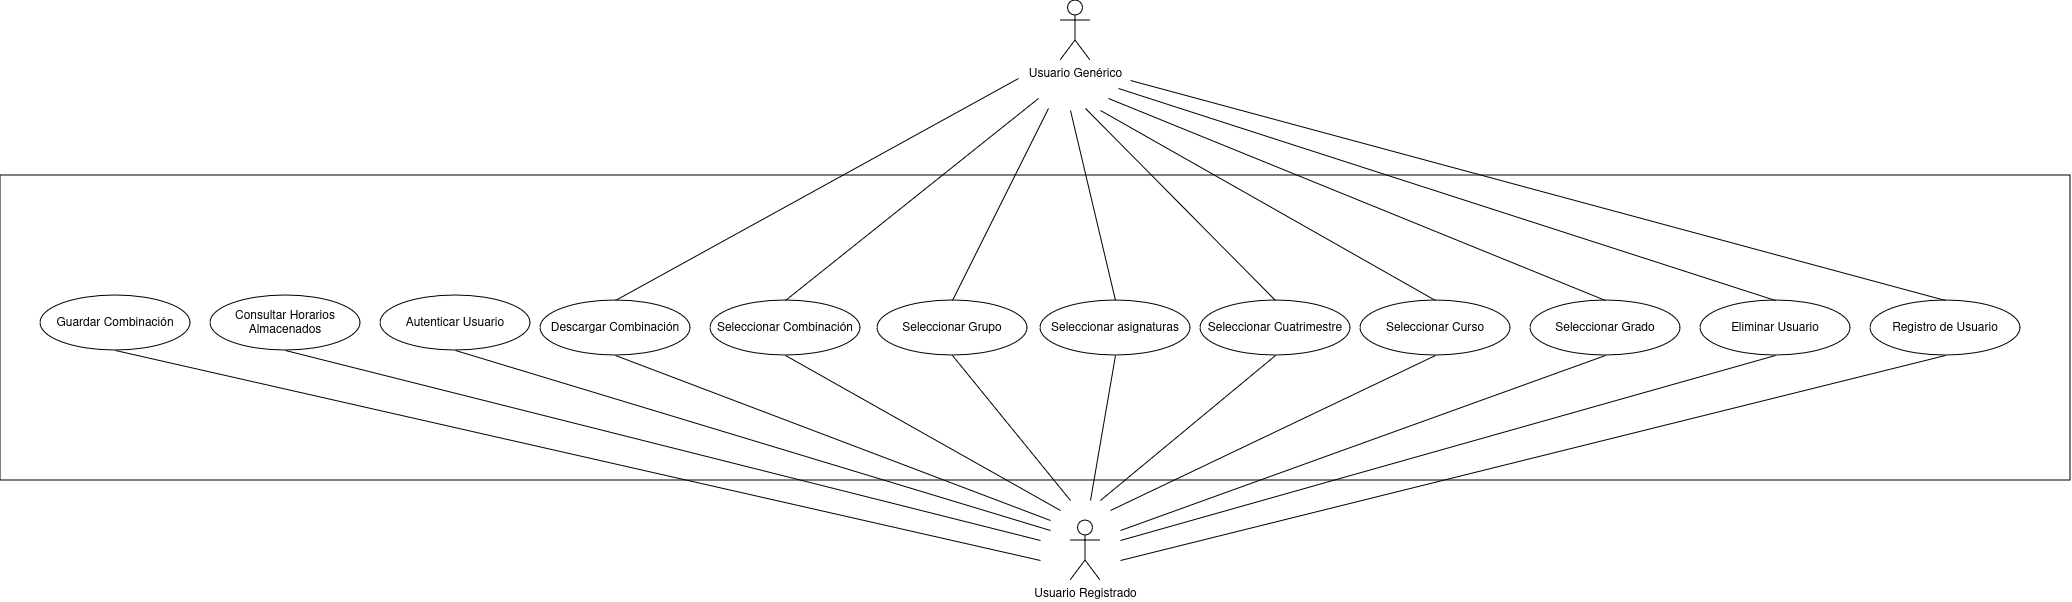
\includegraphics[width=1.9\textwidth]{./imagenes/CC_Actores_Comunes.png}
        \caption{Caso de Uso con Actores Comunes.}
        \label{fig:CC_Actores_Comunes}
    \end{figure}    
\end{landscape}



	% Desarrollo bajo sprints: 
	% 	1. Permitir registros y login de usuarios
	% 	2. Desarrollo del sistema de incidencias
	% 	3. Desarrollo del sistema de denuncias administrativas y accidentes
	% 	4. Desarrollo del sistema de croquis
	%   5. Instalación de la aplicación de manera automática
	\chapter{Implementación}

En esta sección se describen las diferentes etapas que se han llevado a cabo durante el desarrollo del proyecto, los problemas encontrados y las soluciones propuestas. Se incluyen esquemas, capturas de código y ejemplos de uso de la aplicación.\newline

\section{Preparación del entorno de desarrollo}

Previo al comienzo de la implementación, se realizó la configuración del entorno de desarrollo. Esto incluye la instalación de todas las dependecias necesarias, así como las herramientas mencionadas en la sección de diseño.

	% Presupuesto

	% Conclusiones
	\chapter{Conclusiones y trabajos futuros}



	% Trabajos futuros


	
	\newpage
	\bibliography{bibliografia}
	\bibliographystyle{plain}
	
\end{document}

